\documentclass[12pt]{report}
\usepackage{libertine}

% General packages:
\usepackage[utf8]{inputenc}    % Input encoding
\usepackage[T1]{fontenc}       % Font encoding
\usepackage[british]{babel}    % Naming of figures and such
\usepackage[british]{isodate}  % Formatting of dates
\cleanlookdateon               % Show dates cleanly.
%\usepackage{xurl}              % Allow line breaks anywhere in URLs.
\usepackage{minted}            % Needs to be loaded before `csquotes`.
\usepackage[
    citestyle    = authoryear,
    bibstyle     = authoryear,
    giveninits   = true,
    uniquename   = init,
    uniquelist   = false,
    sortlocale   = en_GB,
    backend      = biber,
    backref      = true,
    maxbibnames  = 100,
    maxcitenames = 1,
    dashed       = false,
    % Needed to get sorting right for tussenvoegsels.
    %sortcites    = true,       
    ]{biblatex}                % Bibliography
\usepackage[
    style=american
    ]{csquotes}                % Required for BiBLaTeX
\usepackage{import}            % Importing subdocuments
\usepackage{standalone}        % Compilable subdocuments
% `setspace` needs to be loaded before `hyperref`.
\usepackage{setspace}          % Set line spacing
\usepackage{hyperref}          % Clickable references
\usepackage{microtype}         % Nice typography
\usepackage{makeidx}           % Make an index
\usepackage{silence}           % Silence warnings and errors
\WarningFilter{remreset}{The remreset package}
\WarningFilter*[parskip]{latex}{Command}

% Set line spacing.
\setstretch{1.25}

% Page layout:
\usepackage{tocloft}         % Control ToC
\usepackage[
    a4paper,
    bottom     = 1.1in,
    top        = 1.1in,
    left       = 1.1in,
    right      = 1.1in,
    headheight = 15pt,
    footskip   = 1.5\baselineskip
    ]{geometry}              % Margins
\usepackage{fancyhdr}        % Header
\usepackage{lastpage}        % Page numbers in footer
\usepackage{setspace}        % Line spacing
\usepackage{ragged2e}        % Better line endings
\ActivateWarningFilters[parskip]
\usepackage[
    parfill
    ]{parskip}               % Newlines instead of indentation
\DeactivateWarningFilters[parskip]
\usepackage{titlesec}        % Size of sections
\usepackage{titlecaps}       % Automatic capitalisation of titles
\usepackage[
    hang,
    bottom
    ]{footmisc}              % Configure footnotes
\usepackage{afterpage}       % Include stuff after the current page
\usepackage{placeins}        % Things like `\FloatBarrier`
\usepackage{pdflscape}       % Turn pages sideways
\usepackage{emptypage}       % Remove pagenumbers on empty pages

% Utility:
\usepackage[table]{xcolor}   % Colours
\usepackage[
    separate-uncertainty=true,
    per-mode=symbol
    ]{siunitx}               % Display units
\usepackage{enumitem}        % Better enumeration
\usepackage{xifthen}         % If statements
\usepackage{xpatch}          % Patch things
\usepackage{lipsum}          % Dummy text
\usepackage{listings}        % Listings
\usepackage{xparse}          % Better arguments for \newcommand
\usepackage{xfrac}           % Better fractions
\usepackage{etoolbox}        % Patch stuff
\usepackage[
    notquote
    ]{hanging}               % Hanging paragraphs
\usepackage{scalerel}        % Scale objects
\usepackage{soul}            % Highlighting

% Figures:
\usepackage{pgfplots}        % Plots
\pgfplotsset{compat=newest}
\usepackage{tikz}            % TikZ figures
\usepackage{float}           % Control floating of figures
\usepackage{multirow}        % Cells spanning multiple rows
\usepackage{graphicx}        % Graphics
\usepackage{caption}         % Subfigures and captions
\usepackage{subcaption}      % Subfigures and captions
\usepackage{booktabs}        % Nice looking tables
\usepackage{tabularx}        % Extended functionality for tables

% Math:
\usepackage{amsmath}         % Math
\usepackage{amssymb}         % Math symbols
\usepackage{mathtools}       % Math tools
\usepackage{amsthm}          % Theorems
\usepackage{thmtools}        % More math theorems
\usepackage{bm}              % Bold math symbols
\usepackage{bbm}             % More bold math symbols
\usepackage{cancel}          % Cancel equations
\usepackage{upgreek}         % Upright greek symbols
\usepackage[
    artemisia
    ]{textgreek}             % Greek symbols in text

% This package should be loaded last.
\usepackage[
    noabbrev,
    capitalize,
    nameinlink]{cleveref}    % Automatic referencing

% Add a comma in the cite style.
\renewcommand*{\nameyeardelim}{\addcomma\space}

% Make sure that every `\citeyear` also prints the disambiguating `extradate`.
\DeclareCiteCommand{\citeyearlabel}
    {\usebibmacro{prenote}}
    {\printfield{year}\printfield{extradate}}
    {\multicitedelim}
    {\usebibmacro{postnote}}
\let\citeyearold\citeyear
\let\citeyear\citeyearlabel
\let\citeyearnolabel\citeyearold

% Define a standard for citing within theorem statements.
\newcommand{\theoremcite}[1]{\citeauthor{#1}, \citeyear{#1}}

\newcommand{\fulltextcite}[1]{%
    \AtNextCite{\AtEachCitekey{\defcounter{maxnames}{999}}}%
    \textcite{#1}%
}
\newcommand{\fullparencite}[1]{%
    \AtNextCite{\AtEachCitekey{\defcounter{maxnames}{999}}}%
    \parencite{#1}%
}

% Remove the colon after "In" in the bibliograhpy.
\renewbibmacro*{in:}{\bibstring{in} }

% Tune the electronic print field.
\DeclareFieldFormat{eprint}{%
  \iffieldundef{eprinttype}
    {Electronic print}
    {\thefield{eprinttype}}%
  \addcolon\space
  \ifhyperref
    {\url{#1}}
    {\nolinkurl{#1}}%
  \iffieldundef{eprintclass}
    {}
    {\addspace\mkbibparens{\thefield{eprintclass}}}\printtext{.}}

% Tune URL.
\DeclareFieldFormat{url}{\mkbibacro{URL}\addcolon\space\url{#1}\printtext{.}}

% Tune DOI.
\DeclareFieldFormat{doi}{%
  \mkbibacro{DOI}\addcolon\space
  \ifhyperref
    {\href{https://doi.org/#1}{\nolinkurl{#1}}}
    {\nolinkurl{#1}}\printtext{.}}

% In the below, we will redefine `\finentry` to not print a period if
%` pageref` exists. The period is then added back by `pageref`, but before the
% parentheses. Problems occur when `urldate` is also defined. In that case, 
% the extra period by `pageref` will add a period after `urldate`s
% parentheses, which we do not want. We use the toggle `printperiod` to detect
% this case.

% Tune "visited on".
\DeclareFieldFormat{urldate}{\mkbibparens{\bibstring{urlseen}\space#1\printtext{.}}}
\newtoggle{printperiod}
\toggletrue{printperiod}
\AtBeginBibliography{\renewbibmacro*{urldate}{\printurldate\togglefalse{printperiod}}}

% Tune "cited on".
\renewbibmacro*{finentry}{\iflistundef{pageref}{}{\renewcommand{\finentrypunct}{}}\finentry}
\renewbibmacro*{pageref}{%
  \iflistundef{pageref}
    {}
    {\iftoggle{printperiod}{\setunit{\adddot\addspace}}{}\toggletrue{printperiod}\printtext[parens]{%
       \ifnumgreater{\value{pageref}}{1}
         {\bibstring{backrefpages}\ppspace}
         {\bibstring{backrefpage}\ppspace}%
          \printlist[pageref][-\value{listtotal}]{pageref}.}}}

% Add Oxford comma.
\DefineBibliographyExtras{british}{\def\finalandcomma{\addcomma}}

% Don't abbreviate the backreferences.
\DefineBibliographyStrings{english}{%
    backrefpage = {Cited on page},
    backrefpages = {Cited on pages}
}

% Get tussenvoegsels right. This is not a perfect solution, because the
% in-text citations will be sorted as if the tussenvoegsel is part of the
% last name.
\makeatletter
\AtBeginDocument{\toggletrue{blx@useprefix}}
\AtBeginBibliography{\togglefalse{blx@useprefix}}
\makeatother

% Make an index.
\makeindex

% Show the page number in the bottom center.
\fancypagestyle{plain}{
    \fancyhf{}                          % Clear all header and footers.
    \renewcommand{\headrulewidth}{0pt}  % Remove the header rule.
    \cfoot{\thepage}                    % Show page number in the center.
}
\pagestyle{plain}

% Chapter styling from https://texblog.org/2012/07/03/fancy-latex-chapter-styles/
\newcommand{\hsp}{\hspace{20pt}}
\titleformat{\chapter}[hang]
    {\Huge\bfseries}
    {\thechapter\hsp\textcolor{gray75}{|}\hsp}
    {0pt}
    {\Huge\bfseries}
\titleformat{\section}
    {\normalfont\Large\bfseries\raggedright}
    {\thesection}
    {1em}
    {}
\titleformat{\subsection}
    {\normalfont\large\bfseries\raggedright}
    {\thesubsection}
    {1em}
    {}

% Set spacing after chapter equal to spacing right before section. Then
% things look nicely aligned.
\titlespacing{\chapter}{0pt}{3.5ex}{3.5ex}

% Define the styling of paragraphs.
\renewcommand{\paragraph}[1]{\textbf{#1.}}

% Redefine abstract environment.
\renewenvironment{abstract}
    {\begingroup
    \setstretch{1.25}
    \begin{center}
        \textbf{Abstract}
    \end{center}}
    {\par
    \endgroup}

% Kill any use of the \cite command.
\renewcommand{\cite}[1]{\PackageError{thesis}{use either parencite or authorcite}{}}

% Configure captions.
\WarningFilter{caption}{Unused \captionsetup}
\captionsetup[table]{font=small}
\captionsetup[figure]{font=small}

% Shortcuts for writing.
\newcommand{\ie}{\textit{i.e.}}
\newcommand{\Ie}{\textit{I.e.}}
\newcommand{\eg}{\textit{e.g.}}
\newcommand{\Eg}{\textit{E.g.}}
\newcommand{\cf}{\textit{c.f.}}
\newcommand{\Cf}{\textit{C.f.}}

% \ifempty command:
\newcommand{\ifempty}[3]{\ifthenelse{\equal{#1}{}}{#2}{#3}}

% Style footnotes.
\setlength{\skip\footins}{\baselineskip}
\setlength{\footnotesep}{.75\baselineskip}
\renewcommand{\footnotelayout}{\setstretch{1.0}}
\setlength{\footnotemargin}{1em}

% Typewriter font:
\renewcommand*{\ttdefault}{pcr}  % Courier
\newcommand{\code}[1]{{\small\texttt{#1}}}

% Define some colours.
\definecolor{darkblue} {rgb} {0.0 , 0.0 , 0.65}
\definecolor{darkred}  {rgb} {0.80, 0.0 , 0.0 }
\definecolor{redaccent}{HTML}{E64C66}
\definecolor{darkgreen}{rgb} {0.0 , 0.50, 0.0 }
\definecolor{gray75}   {gray}{0.75}

% Define shortcuts for colours.
\newcommand{\red}[1]{{\color{red} #1}}
\newcommand{\blue}[1]{{\color{blue} #1}}
\newcommand{\green}[1]{{\color{green} #1}}
\newcommand{\orange}[1]{{\color{orange} #1}}
\newcommand{\darkred}[1]{{\color{darkred} #1}}
\newcommand{\darkblue}[1]{{\color{darkblue} #1}}
\newcommand{\darkgreen}[1]{{\color{darkgreen} #1}}
\newcommand{\magenta}[1]{{\color{magenta} #1}}
\newcommand{\grey}[1]{{\color{gray} #1}}

% Use colours to define checkmarks and crosses.
\usepackage{pifont}
\newcommand{\xmark}{\text{\ding{55}}}
\newcommand{\cmark}{\text{\ding{51}}}
\newcommand{\good}{\darkgreen{$\checkmark$}}
\newcommand{\mediumgood}{\orange{$\checkmark$}}
\newcommand{\mediumbad}{\orange{\xmark}}
\newcommand{\bad}{\darkred{\xmark}}

% Load TikZ libraries.
\usetikzlibrary{
    calc,
    positioning,
    fit,
    tikzmark,
    arrows.meta,
    shapes,
    decorations.pathreplacing,
    intersections,
    through
}
% Graphical models:
\tikzset{
    line/.style = {
        thick,
        ->,
        > = {
            Triangle[length=1.5mm, width=1.5mm]
        }
    },
    arrow/.style = {
        line
    },
    % Invisible node:
    hidden node/.style = {
        circle,
        minimum size = 1cm,
        draw = white,
        thick
    },
    % Latent variable:
    latent node/.style = {
        hidden node,
        draw = black,
    },
    % Latent variable:
    factor node/.style = {
        hidden node,
        rectangle,
        draw = black,
    },
    % Observed variable:
    observed node/.style = {
        latent node,
        fill = gray!15
    },
    % Plate:
    plate/.style = {
        draw,
        label={[anchor=north west]south west:#1},
        rounded corners=2pt,
        shape=rectangle,
        inner sep=10pt,
        thick
    }
}

% Circled number:
\newcommand{\ballnumber}[1]{%
    \tikz[baseline=(n.base)] \node[circle,fill=.,inner sep=1pt,text=white] (n) {\normalshape\bfseries\footnotesize #1};%
}
\newcommand{\itemballnumber}[1]{%
    \raisebox{.5pt}{\ballnumber{#1}}%
}

% Style enumerate and lists. Do not use `label=(\arabic*)` because equation
% numbering already uses the same style.
\setenumerate{topsep=.25\baselineskip, itemsep=0pt}
\setlist{topsep=.25\baselineskip, itemsep=0pt}
% \setlist[enumerate]{
%     label=(\arabic*),
%     itemsep=-0.25\baselineskip,
%     topsep=0.25\baselineskip,
%     after={\vspace*{0.25\baselineskip}}
% }
% \setlist[enumerate,2]{
%     topsep=-0.25\baselineskip,
%     itemsep=0pt,
%     label=(\alph*)
% }
% \setlist[enumerate,3]{
%     topsep=-0.25\baselineskip,
%     itemsep=0pt,
%     label=(\roman*)
% }
% \setlist[itemize]{
%     label=\textbullet,
%     itemsep=-0.25\baselineskip,
%     topsep=0.25\baselineskip
% }
% \setlist[itemize,2]{
%     topsep=-0.25\baselineskip,
%     itemsep=0pt
% }
% \setlist[itemize,3]{
%     topsep=-0.25\baselineskip,
%     itemsep=0pt
% }

% Set the default float placement correctly.
\floatplacement{figure}{tbp}
\floatplacement{table}{tbp}

% Set spacing between figures and text.
\setlength{\textfloatsep}{30pt plus 1.0pt minus 2.0pt}
\setlength{\floatsep}{30pt plus 1.0pt minus 2.0pt}
\setlength{\intextsep}{30pt plus 1.0pt minus 2.0pt}

% Adjust line spacing in captions.
\captionsetup{font={stretch=1.25}}

% Newline for in a title.
\newcommand{\tnl}{\texorpdfstring{\\}{}}

% Define outline tools.
\newcommand{\outline}[1]{
    \parbox{\linewidth}{
        \setstretch{1.0}
        \color{darkgreen}
        #1
    }\vspace{\parskip}
}
\newlist{outlinelist}{enumerate}{1}
\setlist[outlinelist]{
    label=\arabic*.,
    noitemsep,
    topsep=0pt,
    parsep=0pt,
    partopsep=0pt
}
\newcommand{\note}[1]{{\color{darkred}#1}}

% Left-justified text in tabularx environment:
\newcolumntype{L}{>{\RaggedRight\arraybackslash}X}

% Hyperlink setup.
\hypersetup{
    colorlinks,
    citecolor = black,
    filecolor = black,
    linkcolor = black,
    urlcolor  = black
}

% Landscape figures:
\newcommand{\landscapefloat}[1]{
    \afterpage{
        \begin{landscape}
            #1
        \end{landscape}
    }
}

% Hanging full citation:
\newcommand{\hangcite}[1]{\hangpara{\bibhang}{1}\AtNextCite{\defcounter{maxnames}{99}}\fullcite{#1}}

% Define \charfusion. From https://tex.stackexchange.com/a/52673.
\makeatletter
\def\moverlay{\mathpalette\mov@rlay}
\def\mov@rlay#1#2{\leavevmode\vtop{%
   \baselineskip\z@skip \lineskiplimit-\maxdimen
   \ialign{\hfil$\m@th#1##$\hfil\cr#2\crcr}}}
    \newcommand{\charfusion}[3][\mathord]{
        #1{\ifx#1\mathop\vphantom{#2}\fi
        \mathpalette\mov@rlay{#2\cr#3}}
        \ifx#1\mathop\expandafter\displaylimits\fi
    }
\makeatother

% Sha symbol.
%   Source: https://tex.stackexchange.com/questions/124738/i-just-want-to-write-sha-without-ruining-everything
\DeclareFontFamily{U}{wncy}{}
\DeclareFontShape{U}{wncy}{m}{n}{<->wncyr10}{}
\DeclareSymbolFont{mcy}{U}{wncy}{m}{n}
\DeclareMathSymbol{\Sha}{\mathord}{mcy}{"58}

% Define a bigger \cdot.
%   Source: https://tex.stackexchange.com/questions/235118/making-a-thicker-cdot-for-dot-product-that-is-thinner-than-bullet
\makeatletter
\newcommand*\bigcdot{\mathpalette\bigcdot@{.5}}
\newcommand*\bigcdot@[2]{\mathbin{\vcenter{\hbox{\scalebox{#2}{$\m@th#1\bullet$}}}}}
\makeatother

% Bold math symbols from text greeks:
\newcommand{\mathbfup}[1]{\mathord{\textnormal{\textbf{#1}}}}

% Bold characters:
\renewcommand{\vec}[1]{\boldsymbol{#1}}
\newcommand{\vecu}[1]{\hat{\vec{#1}}}
\newcommand{\mat}[1]{\vec{#1}}

% Predefined matrices and vectors:
\newcommand{\vnull}{\mathbf{0}}

\newcommand{\va}{\mathbf{a}}
\newcommand{\vb}{\mathbf{b}}
\newcommand{\vc}{\mathbf{c}}
\newcommand{\vd}{\mathbf{d}}
\newcommand{\ve}{\mathbf{e}}
\newcommand{\vf}{\mathbf{f}}
\newcommand{\vg}{\mathbf{g}}
\newcommand{\vh}{\mathbf{h}}
\newcommand{\vi}{\mathbf{i}}
\newcommand{\vj}{\mathbf{j}}
\newcommand{\vk}{\mathbf{k}}
\newcommand{\vl}{\mathbf{l}}
\newcommand{\vm}{\mathbf{m}}
\newcommand{\vn}{\mathbf{n}}
\newcommand{\vo}{\mathbf{o}}
\newcommand{\vp}{\mathbf{p}}
\newcommand{\vq}{\mathbf{q}}
\newcommand{\vr}{\mathbf{r}}
\newcommand{\vs}{\mathbf{s}}
\newcommand{\vt}{\mathbf{t}}
\newcommand{\vu}{\mathbf{u}}
\newcommand{\vv}{\mathbf{v}}
\newcommand{\vw}{\mathbf{w}}
\newcommand{\vx}{\mathbf{x}}
\newcommand{\vy}{\mathbf{y}}
\newcommand{\vz}{\mathbf{z}}

% Must be enclosed in another group.
\newcommand{\vmu}{{\mathbfup{\textmu}}}
\newcommand{\vtheta}{{\bm{\uptheta}}}
\newcommand{\vphi}{{\mathbfup{\textphi}}}
\newcommand{\vtau}{{\mathbfup{\texttau}}}
\newcommand{\vep}{{\mathbfup{\textepsilon}}}
\newcommand{\vth}{{\mathbfup{\texttheta}}}

\newcommand{\mA}{\mathbf{A}}
\newcommand{\mB}{\mathbf{B}}
\newcommand{\mC}{\mathbf{C}}
\newcommand{\mD}{\mathbf{D}}
\newcommand{\mE}{\mathbf{E}}
\newcommand{\mF}{\mathbf{F}}
\newcommand{\mG}{\mathbf{G}}
\newcommand{\mH}{\mathbf{H}}
\newcommand{\mI}{\mathbf{I}}
\newcommand{\mJ}{\mathbf{J}}
\newcommand{\mK}{\mathbf{K}}
\newcommand{\mL}{\mathbf{L}}
\newcommand{\mM}{\mathbf{M}}
\newcommand{\mN}{\mathbf{N}}
\newcommand{\mO}{\mathbf{O}}
\newcommand{\mP}{\mathbf{P}}
\newcommand{\mQ}{\mathbf{Q}}
\newcommand{\mR}{\mathbf{R}}
\newcommand{\mS}{\mathbf{S}}
\newcommand{\mT}{\mathbf{T}}
\newcommand{\mU}{\mathbf{U}}
\newcommand{\mV}{\mathbf{V}}
\newcommand{\mW}{\mathbf{W}}
\newcommand{\mX}{\mathbf{X}}
\newcommand{\mY}{\mathbf{Y}}
\newcommand{\mZ}{\mathbf{Z}}

\newcommand{\mSigma}{\mathbfup{\textSigma}}

% Letters commonly used in blackboard bold font:
\newcommand{\Ab}{\mathbb{A}}
\newcommand{\Bb}{\mathbb{B}}
\newcommand{\Db}{\mathbb{D}}
\newcommand{\C}{\mathbb{C}}
\newcommand{\E}{\mathbb{E}}
\newcommand{\Hb}{\mathbb{H}}
\newcommand{\Jb}{\mathbb{J}}
\newcommand{\K}{\mathbb{K}}
\newcommand{\Lb}{\mathbb{L}}
\newcommand{\Mb}{\mathbb{M}}
\newcommand{\N}{\mathbb{N}}
\renewcommand{\P}{\mathbb{P}}
\newcommand{\Q}{\mathbb{Q}}
\newcommand{\R}{\mathbb{R}}
\newcommand{\eR}{\overline{\mathbb{R}}}
\newcommand{\Sb}{\mathbb{S}}
\newcommand{\Tb}{\mathbb{T}}
\newcommand{\V}{\mathbb{V}}
\newcommand{\Z}{\mathbb{Z}}

% Letters commonly used in calligraphic font:
\newcommand{\A}{\mathcal{A}}
\newcommand{\B}{\mathcal{B}}
\newcommand{\Cc}{\mathcal{C}}
\newcommand{\D}{\mathcal{D}}
\newcommand{\Ec}{\mathcal{E}}
\newcommand{\F}{\mathcal{F}}
\newcommand{\G}{\mathcal{G}}
\let\Haccent\H
\renewcommand{\H}{\mathcal{H}}
\newcommand{\J}{\mathcal{J}}
\newcommand{\Jrat}{\mathcal{J}_{\text{rat}}}
\newcommand{\Kc}{\mathcal{K}}
\renewcommand{\L}{\mathcal{L}}
\newcommand{\Li}{\mathcal{L}{}^1}
\newcommand{\eLi}{\overline{\mathcal{L}}{}^1}
\newcommand{\m}{\text{m}}
\newcommand{\M}{\mathcal{M}}
\newcommand{\eM}{\overline{\mathcal{M}}}
\newcommand{\Nc}{\mathcal{N}}
\newcommand{\Oc}{\mathcal{O}}
\newcommand{\Pc}{\mathcal{P}}
\newcommand{\Qc}{\mathcal{Q}}
\newcommand{\Rc}{\mathcal{R}}
\renewcommand{\S}{\mathcal{S}}
\newcommand{\Tc}{\mathcal{T}}
\newcommand{\U}{\mathcal{U}}
\newcommand{\Vc}{\mathcal{V}}
\newcommand{\W}{\mathcal{W}}
\newcommand{\X}{\mathcal{X}}
\newcommand{\Y}{\mathcal{Y}}
\newcommand{\Zc}{\mathcal{Z}}

% Letters sometimes used with a wide tilde:
\newcommand{\tpi}{\widetilde{\pi}}
\newcommand{\ttau}{\widetilde{\tau}}
\newcommand{\tvtau}{\widetilde{\vtau}}
\newcommand{\tD}{\widetilde{\D}}
\newcommand{\tX}{\widetilde{\X}}
\newcommand{\tI}{\widetilde{I}}
\newcommand{\tQc}{\widetilde{\Qc}}

% Letters commonly used in sans serif font:
\newcommand{\T}{\text{\normalshape\textsf{T}}}
\newcommand{\Ht}{\text{\normalshape\textsf{H}}}
\renewcommand{\c}{\text{\normalshape\textsf{c}}}

% Symbols:
\newcommand{\es}{\varnothing}
\newcommand{\e}{\varepsilon}
\newcommand{\sub}{\subseteq}
\renewcommand{\d}{\partial}
\renewcommand{\th}{\theta}
\newcommand{\Th}{\Theta}

% Substitute l for \ell throughout.
%   Source: https://tex.stackexchange.com/questions/1975/substituting-character-l-with-ell-throughout-math-mode
\mathcode`l="8000
\begingroup
\makeatletter
\lccode`\~=`\l
\DeclareMathSymbol{\lsb@l}{\mathalpha}{letters}{`l}
\lowercase{\gdef~{\ifnum\the\mathgroup=\m@ne \ell \else \lsb@l \fi}}%
\endgroup

% Convergence symbols:
\newcommand{\oto}[1]{\overset{#1}{\to}}
\newcommand{\uto}[1]{\underset{#1}{\to}}
\newcommand{\outo}[2]{\overset{#1}{\underset{#2}{\to}}}
\newcommand{\Lto}[1]{\oto{\L^{#1}}}
\newcommand{\weakto}{\rightharpoonup}
\newcommand{\distto}{\oto{\text{d}}}
\newcommand{\weakstarto}{\overset{\ast}{\rightharpoonup}}
% Big-O notation:
\renewcommand{\O}{O}

% Equality symbols:
\newcommand{\disteq}{\overset{\text{\normalshape d}}{=}}

% Operators:
\DeclareMathOperator*{\argmax}{arg\,max}
\DeclareMathOperator*{\argmin}{arg\,min}
\let\max\relax\DeclareMathOperator*{\max}{max}
\let\min\relax\DeclareMathOperator*{\min}{min}
\let\sup\relax\DeclareMathOperator*{\sup}{sup}
\let\inf\relax\DeclareMathOperator*{\inf}{inf\vphantom{p}}
\let\limsup\relax\DeclareMathOperator*{\limsup}{lim\,sup}
\let\liminf\relax\DeclareMathOperator*{\liminf}{lim\,inf\vphantom{p}}
\DeclareMathOperator*{\esssup}{ess\,sup}
\DeclareMathOperator*{\essinf}{ess\,inf}
\newcommand{\AC}{\operatorname{AC}}
\newcommand{\atan}{\operatorname{atan}}
\newcommand{\Breg}{\operatorname{D}}
\newcommand{\BV}{\operatorname{BV}}
\newcommand{\card}{\#}
\newcommand{\cconv}{\circledast}
\newcommand{\chol}{\operatorname{chol}}
\newcommand{\ch}{\operatorname{ch}}
\newcommand{\cliques}{\operatorname{cliques}}
\newcommand{\cl}{\operatorname{cl}}
\newcommand{\col}{\operatorname{col}}
\newcommand{\comp}{\circ}
\newcommand{\contains}{\supseteq}
\newcommand{\conv}{\ast}
\newcommand{\cov}{\operatorname{cov}}
\newcommand{\var}{\operatorname{var}}
\renewcommand{\deg}{\operatorname{deg}}
\renewcommand{\det}{\operatorname{det}}
\newcommand{\diag}{\operatorname{diag}}
\renewcommand{\dim}{\operatorname{dim}}
\newcommand{\diam}{\operatorname{diam}}
\renewcommand{\div}{\operatorname{div}}
\newcommand{\dist}{\operatorname{dist}}
\newcommand{\dom}{\operatorname{dom}}
\newcommand{\dotcup}{\charfusion[\mathbin]{\cup}{\cdot}}
\newcommand{\dotunion}{\charfusion[\mathop]{\bigcup}{\cdot}}
\newcommand{\dsum}{\oplus}
\newcommand{\Dsum}{\bigoplus}
\newcommand{\erf}{\operatorname{erf}}
\newcommand{\epi}{\operatorname{epi}}
\newcommand{\had}{\odot}
\newcommand{\Hell}{\operatorname{D}_{\text{Hell}}}
\newcommand{\hypo}{\operatorname{hypo}}
\newcommand{\im}{\operatorname{im}}
\renewcommand{\Im}{\operatorname{Im}}
\newcommand{\ind}{\mathbbm{1}}
\newcommand{\intersection}{\bigcap}
\newcommand{\join}{\lor}
\newcommand{\KL}{\operatorname{KL}}
\newcommand{\KOT}{\operatorname{KOT}}
\newcommand{\kron}{\otimes}
\newcommand{\len}{\operatorname{len}}
\newcommand{\Lip}{\operatorname{Lip}}
\newcommand{\meet}{\land}
\newcommand{\MOT}{\operatorname{MOT}}
\newcommand{\nullspace}{\operatorname{null}}
\newcommand{\Per}{\operatorname{Per}}
\newcommand{\push}{_\#}
\newcommand{\poly}{\operatorname{poly}}
\newcommand{\rank}{\operatorname{rank}}
\renewcommand{\Re}{\operatorname{Re}}
\newcommand{\row}{\operatorname{row}}
\newcommand{\schur}{\operatorname{Schur}}
\newcommand{\sign}{\operatorname{sign}}
\newcommand{\sinth}{\operatorname{\sin\!\text{-}\Theta}}
\newcommand{\Sinth}{\operatorname{\text{Sin-}\Theta}}
\newcommand{\supp}{\operatorname{supp}}
\newcommand{\symdiff}{\bigtriangleup}
\newcommand{\Tan}{\operatorname{Tan}}
\newcommand{\tensor}{\otimes}
\newcommand{\TV}{\operatorname{TV}}
\newcommand{\tr}{\operatorname{tr}}
\newcommand{\union}{\bigcup}
\newcommand{\vecspan}{\operatorname{span}}
\newcommand{\vect}{\operatorname{vec}}
\newcommand{\vol}{\operatorname{vol}}

% Probability distributions:
\newcommand{\Ber}{\operatorname{Ber}}
\newcommand{\Beta}{\operatorname{Beta}}
\newcommand{\Bin}{\operatorname{Bin}}
\newcommand{\BM}{\operatorname{BM}}
\newcommand{\Cat}{\operatorname{Cat}}
\newcommand{\Cauchy}{\operatorname{Cauchy}}
\newcommand{\Dir}{\operatorname{Dir}}
\newcommand{\Exp}{\operatorname{Exp}}
\newcommand{\Gam}{\operatorname{Gamma}}
\newcommand{\Geom}{\operatorname{Geom}}
\newcommand{\GP}{\mathcal{GP}}
\newcommand{\InvWishart}{\mathcal{W}^{-1}}
\newcommand{\Laplace}{\operatorname{Laplace}}
\newcommand{\LogNormal}{\log\mathcal{N}}
\newcommand{\Mult}{\operatorname{Mult}}
\newcommand{\NegBin}{\operatorname{NegBin}}
\newcommand{\Normal}{\mathcal{N}}
\newcommand{\Poisson}{\operatorname{Poisson}}
\newcommand{\Rad}{\operatorname{Rad}}
\newcommand{\Unif}{\operatorname{Unif}}
\newcommand{\Wishart}{\mathcal{W}}
\newcommand{\WN}{\operatorname{WN}}

\newcommand{\simiid}{\overset{\text{i.i.d.}}{\sim}}

% Probability commands:
\newcommand{\Var}{\V}
\newcommand{\Lik}{\L}
\newcommand{\iidsim}{\overset{\text{\tiny{i.i.d.}}}{\sim}}

% Special math commands:
\newcommand{\cond}{\,|\,}                  % Conditioning
\newcommand{\middlecond}{\,\middle|\,}     % Conditioning between a \left and \right
\newcommand{\divsep}{\,\|\,}               % Separator in divergences
\newcommand{\middledivsep}{\,\middle\|\,}  % Separator in divergences ebtween a \left and a \right

\newcommand{\sd}[1]{\mathrm{d} #1}         % Straight 'd'
\newcommand{\isd}[1]{\, \mathrm{d} #1}     % Straight 'd' in integral (with spacing)
% Straight 'd' in integral with spacing and absolute value around it
\newcommand{\asd}[1]{\, |\mathrm{d} #1|}

\newcommand{\idf}{\text{\textsf{id}}}            % Identity function
\newcommand{\sce}{\text{\sc{e}}}                 % Scientific notation
\newcommand{\vardot}{\,\bigcdot\,}               % Variable dot
\let\ssorig\ss
\renewcommand{\ss}[1]{_{\text{\normalshape #1}}} % Text subscripts
\newcommand{\us}[1]{^{\text{\normalshape #1}}}   % Text superscripts

% Hard to type words:
\newcommand{\cadlag}{c\`adl\`ag}
\newcommand{\Cadlag}{C\`adl\`ag}
\newcommand{\ito}{It\^o}
\newcommand{\Ito}{\ito}
\newcommand{\levy}{L\`evy}
\newcommand{\Levy}{\levy}

% Subscripts
\newcommand{\loc}{_{\text{loc}}}
\newcommand{\lip}{_{\text{Lip}}}

% Half rectangle:
\newcommand{\halfrect}[2]{[\![#1,#2)\hspace{-1pt}\!)}
\newcommand{\Rint}{\text{(R)}\int}

% Paired delimiters:
\DeclarePairedDelimiter\parens{(}{)}             % Parentheses
\DeclarePairedDelimiter\sbrac{[}{]}              % Square brackets
\DeclarePairedDelimiter\cbrac{\{}{\}}            % Curly braces
\DeclarePairedDelimiter\set{\{}{\}}              % Set
\DeclarePairedDelimiter\lra{\langle}{\rangle}    % Angle brackets
\DeclarePairedDelimiter\dlra
    {\langle\!\langle}{\rangle\!\rangle}         % Double angle brackets
\DeclarePairedDelimiter\floor{\lfloor}{\rfloor}  % Floor
\DeclarePairedDelimiter\ceil{\lceil}{\rceil}     % Ceil
\DeclarePairedDelimiter\norm{\|}{\|}             % Norm
\DeclarePairedDelimiter\abs{|}{|}                % Absolute value

% Shortcuts for angle brackets:
\newcommand{\la}{\langle}
\newcommand{\ra}{\rangle}
\newcommand{\lla}{\left\langle}
\newcommand{\rra}{\right\rangle}

% Other commands:
\newcommand{\resp}[1]{[#1]}                  % Respective statement
\newcommand{\bs}{\textbackslash}             % Blackslash in text
% Use \cref in a title.
\newcommand{\creftitle}[2]{\texorpdfstring{\cref{#2}}{#1 \ref{#2}}}
\newcommand{\mcheckthis}{{}^{[\checkmark]}}  % Checkmark in math
\newcommand{\checkthis}{$\mcheckthis$}       % Checkmark in text

% Compatibility with old commands:
\newcommand{\id}[1]{\sd{#1}}
\newcommand{\sargmax}[1]{\argmin_{#1}}
\newcommand{\sargmin}[1]{\argmax_{#1}}
\newcommand{\lrset}[1]{\set*{#1}}
\newcommand{\middleCond}{\middlecond}
\newcommand{\rel}[2]{($(#1) + (#2)$)}
\newcommand{\blackLinks}{}
\newcommand{\Ac}{\A}

\newcommand{\notheorems}{}  % We'll configure our own numbering below.
% Patch \listoftheorems.
%   Source: https://tex.stackexchange.com/questions/249963/remove-repeated-theorem-in-the-list-of-theorems
\makeatletter
\patchcmd\thmt@mklistcmd
    {\thmt@thmname}
    {\check@optarg{\thmt@thmname}}
    {}{}
\patchcmd\thmt@mklistcmd
    {\thmt@thmname\ifx}
    {\check@optarg{\thmt@thmname}\ifx}
    {}{}
\protected\def\check@optarg#1{%
    \@ifnextchar\thmtformatoptarg\@secondoftwo{#1}%
}
\makeatother

% Define lists of things commands.
\let\oldlistoftheorems\listoftheorems
\newcommand{\listofmodels}{
    \renewcommand{\listtheoremname}{List of Models}
    \oldlistoftheorems[ignoreall, show={model}]
}
\newcommand{\listofstatements}{
    \renewcommand{\listtheoremname}{List of Mathematical Statements}
    \oldlistoftheorems[ignoreall, show={theorem,corollary,proposition,lemma,fact}]
}
\renewcommand{\listoftheorems}{
    \renewcommand{\listtheoremname}{List of Theorems}
    \oldlistoftheorems[ignoreall, show={theorem}]
}

% Define environments.
\newlength{\thmtopsep}\setlength{\thmtopsep}{\topsep}
\newlength{\thmbotsep}\setlength{\thmbotsep}{\topsep}
\newtheoremstyle{theoremstyle}
    {\thmtopsep}{\thmbotsep}
    {}           % Body font
    {}           % Indent amount
    {\bfseries}  % Theorem head font
    {.}          % Punctuation after theorem head
    {.5em}       % Space after theorem head
    {}           % Theorem head spec
\theoremstyle{theoremstyle}

\ifcsname notheorems\endcsname
\else
    \newtheorem{theorem}{Theorem}[section]
    \newtheorem{proposition}{Proposition}[section]
    \newtheorem{corollary}{Corollary}[section]
    \newtheorem{fact}{Fact}[section]
    \newtheorem{lemma}{Lemma}[section]

    \newtheorem{assumption}{Assumption}[section]
    \newtheorem{definition}{Definition}[section]
    \newtheorem{question}{Question}[section]
    \newtheorem{example}{Example}[section]
    \newtheorem{model}{Model}[section]
    \newtheorem{remark}{Remark}[section]
\fi

% Set referencing formats.
\crefname{assumption}{Assumption}{Assumptions}
\Crefname{assumption}{Assumption}{Assumptions}
\crefname{corollary}{Corollary}{Corollaries}
\Crefname{corollary}{Corollary}{Corollaries}
\crefname{definition}{Definition}{Definitions}
\Crefname{definition}{Definition}{Definitions}
\crefname{example}{Example}{Examples}
\Crefname{example}{Example}{Examples}
\crefname{fact}{Fact}{Facts}
\Crefname{fact}{Fact}{Facts}
\crefname{lemma}{Lemma}{Lemmas}
\Crefname{lemma}{Lemma}{Lemmas}
\crefname{model}{Model}{Models}
\Crefname{model}{Model}{Models}
\crefname{proposition}{Proposition}{Propositions}
\Crefname{proposition}{Proposition}{Propositions}
\crefname{question}{Question}{Questions}
\Crefname{question}{Question}{Questions}
\crefname{remark}{Remark}{Remarks}
\Crefname{remark}{Remark}{Remarks}
\crefname{theorem}{Theorem}{Theorems}
\Crefname{theorem}{Theorem}{Theorems}

% Referentiable list items in environments
\newlist{asslist}{enumerate}{1}
\setlist[asslist]{
    ref=\theassumption.(\arabic*),
    label=(\arabic*),
    % topsep=0pt,
}
\crefname{asslisti}{Assumption}{Assumptions}
\Crefname{asslisti}{Assumption}{Assumptions}
\newlist{corlist}{enumerate}{1}
\setlist[corlist]{
    ref=\thecorollary.(\arabic*),
    label=(\arabic*),
    % topsep=0pt,
}
\crefname{corlisti}{Corollary}{Corollaries}
\Crefname{corlisti}{Corollary}{Corollaries}
\newlist{deflist}{enumerate}{1}
\setlist[deflist]{
    ref=\thedefinition.(\arabic*),
    label=(\arabic*),
    % topsep=0pt,
}
\crefname{deflisti}{Definition}{Definitions}
\Crefname{deflisti}{Definition}{Definitions}
\newlist{exlist}{enumerate}{1}
\setlist[exlist]{
    ref=\theexample.(\arabic*),
    label=(\arabic*),
    % topsep=0pt,
}
\crefname{exlisti}{Example}{Examples}
\Crefname{exlisti}{Example}{Examples}
\newlist{factlist}{enumerate}{1}
\setlist[factlist]{
    ref=\thefact.(\arabic*),
    label=(\arabic*),
    % topsep=0pt,
}
\crefname{factlisti}{Fact}{Facts}
\Crefname{factlisti}{Fact}{Facts}
\newlist{lemlist}{enumerate}{1}
\setlist[lemlist]{
    ref=\thelemma.(\arabic*),
    label=(\arabic*),
    % topsep=0pt,
}
\crefname{lemlisti}{Lemma}{Lemmas}
\Crefname{lemlisti}{Lemma}{Lemmas}
\newlist{modlist}{enumerate}{1}
\setlist[modlist]{
    ref=\themodel.(\arabic*),
    label=(\arabic*),
    % topsep=0pt,
}
\crefname{modlisti}{Model}{Models}
\Crefname{modlisti}{Model}{Models}
\newlist{proplist}{enumerate}{1}
\setlist[proplist]{
    ref=\theproposition.(\arabic*),
    label=(\arabic*),
    % topsep=0pt,
}
\crefname{proplisti}{Proposition}{Propositions}
\Crefname{proplisti}{Proposition}{Propositions}
\newlist{qlist}{enumerate}{1}
\setlist[qlist]{
    ref=\theremark.(\arabic*),
    label=(\arabic*),
    % topsep=0pt,
}
\crefname{qlisti}{Question}{Questions}
\Crefname{qlisti}{Question}{Questions}
\newlist{remlist}{enumerate}{1}
\setlist[remlist]{
    ref=\theremark.(\arabic*),
    label=(\arabic*),
    % topsep=0pt,
}
\crefname{remlisti}{Remark}{Remarks}
\Crefname{remlisti}{Remark}{Remarks}
\newlist{thmlist}{enumerate}{1}
\setlist[thmlist]{
    ref=\thetheorem.(\arabic*),
    label=(\arabic*),
    % topsep=0pt,
}
\crefname{thmlisti}{Theorem}{Theorems}
\Crefname{thmlisti}{Theorem}{Theorems}

% Reference numbers in the list.
\newcommand{\listnum}[1]{(#1)}
\newcommand{\listimp}[2]{\listnum{#1} $\Rightarrow$ \listnum{#2}}
\newcommand{\listeq}[2]{\listnum{#1} $\Leftrightarrow$ \listnum{#2}}

% Backward compatibility:
\newcommand{\listimpl}[2]{\listnum{#1} $\Rightarrow$ \listnum{#2}:}


% We actually will use coloured links.
\definecolor{aquamarine}{HTML}{218274}
\hypersetup{
    colorlinks,
    citecolor = aquamarine,
    filecolor = aquamarine,
    linkcolor = aquamarine,
    urlcolor  = aquamarine,
}

% Use italic font in bodies for clarity.
\newtheoremstyle{theoremstyle}
    {\thmtopsep}{\thmbotsep}
    {\itshape}   % Body font
    {}           % Indent amount
    {\bfseries}  % Theorem head font
    {.}          % Punctuation after theorem head
    {.5em}       % Space after theorem head
    {}           % Theorem head spec
\theoremstyle{theoremstyle}

% Set numbering of theorems right.
\newtheorem{theorem}{Theorem}[chapter]
\newtheorem{proposition}[theorem]{Proposition}
\newtheorem{corollary}[theorem]{Corollary}
\newtheorem{fact}[theorem]{Fact}
\newtheorem{lemma}[theorem]{Lemma}

\newtheorem{assumption}[theorem]{Assumption}
\newtheorem{definition}[theorem]{Definition}
\newtheorem{procedure}[theorem]{Procedure}

\newtheorem{question}[theorem]{Question}
\newtheorem{example}[theorem]{Example}
\newtheorem{model}[theorem]{Model}
\newtheorem{remark}[theorem]{Remark}

% Hack `\listoftheorem` to remove the title.
\makeatletter
\renewcommand\listoftheorems[1][]{%
    \begingroup
    \setlisttheoremstyle{#1}%
    \let\listfigurename\listtheoremname
    \def\contentsline##1{%
        \csname thmt@contentsline@##1\endcsname{##1}%
    }%
    \@for\thmt@envname:=\thmt@allenvs\do{%
        \thmtlo@newentry
    }%
    \let\thref@starttoc\@starttoc
    \def\@starttoc##1{\thref@starttoc{loe}}%
    \@fileswfalse
    \AtEndDocument{%
        \if@filesw
        \@ifundefined{tf@loe}{%
            \expandafter\newwrite\csname tf@loe\endcsname
            \immediate\openout \csname tf@loe\endcsname \jobname.loe\relax
        }{}%
        \fi
    }%
    \@starttoc{lof}
    \endgroup
}
\makeatother

% Fix spacing around proofs.
\xpatchcmd{\proof}{\topsep6\p@\@plus6\p@\relax}{}{}{}
\BeforeBeginEnvironment{proof}{\vspace{-0.5em}}
\AfterEndEnvironment{proof}{\vspace{-0.5em}}

% Commands specific for thesis:
\newcommand{\AR}{\operatorname{AR}}
\newcommand{\enc}{\mathsf{enc}}
\newcommand{\dec}{\mathsf{dec}}
\newcommand{\mult}{\operatorname{mult}}

\newcommand{\missingcite}{\note{(CITATION MISSING)}}

% Listings:
\usepackage{tcolorbox}
\tcbuselibrary{minted,skins,breakable}

\definecolor{solarized-light-bg}{HTML}{fdf6e3}
\definecolor{solarized-light-fg}{HTML}{586e75}
\newtcblisting{pythoncode}[2]{
    listing engine = minted,
    listing only,
    minted style = solarized-light,
    minted language = python,
    minted options = {
        fontsize = #1,
        escapeinside = ||,
        mathescape = true,
        highlightlines = #2,
        highlightcolor = red,
    },
    colback = solarized-light-bg,
    colframe = solarized-light-bg,
    toprule = 0pt,
    left = 5pt,
    left = 5pt,
    leftrule = 0pt,
    rightrule = 0pt,
    bottomrule = 0pt,
    arc = 0pt,
    frame hidden,
    breakable,
}
% Disable italics.
\AtBeginEnvironment{pythoncode}{\let\itshape\relax}

% Override the textwriter font.
%\usepackage[scaled=0.8]{beramono}
\usepackage[scaled=0.95]{inconsolata}
\renewcommand{\code}[1]{\colorbox{solarized-light-bg}{\small\color{solarized-light-fg}\texttt{#1}}}

% We never want footnotes to break across pages.
\interfootnotelinepenalty=10000

% Allow restatable environments.
\newenvironment{manual}[3][]{%
    \def\savedarg{#2}%
    \expandafter\renewcommand\csname the#2\endcsname{#3}%
    \ifempty{#1}{\csname #2\endcsname}{\csname #2\endcsname[#1]}%
}{%
    \csname end\savedarg\endcsname%
    \addtocounter{\savedarg}{-1}%
}
\newcommand{\statement}[1]{
    \begingroup
        \subimport{}{#1}
        \ifempty{\statementoption}{
            \csname\statementtype\endcsname
        }{
            \expandafter\csname\statementtype\endcsname[\statementoption]%
        }
        \label{\statementlabel}
        \statementcontent
        \csname end\statementtype\endcsname
    \endgroup
}
\newcommand{\restatement}[1]{
    \begingroup
        \subimport{}{#1}
        \ifempty{\statementoption}{
            \manual{\statementtype}{\ref{\xrprefix{\statementlabel}}}
        }{
            \manual[\statementoption]{\statementtype}{\ref{\xrprefix{\statementlabel}}}
        }
        \newcommand{\insiderestatement}{}
        \renewcommand{\label}[1]{}
        \statementcontent
        \endmanual
    \endgroup
}

%\newcommand{\ballnumber}[1]{\tikz[baseline=(myanchor.base)] \node[circle,fill=.,inner sep=1pt] (myanchor) {\color{-.}\normalshape\bfseries\footnotesize #1};}

\newcommand{\highlight}{\textcolor{}{}}

\addbibresource{../../bibliography.bib}

\usepackage{xr}
\externaldocument[xr-]{../../main}
\newcommand{\xrprefix}[1]{xr-#1}

\newcommand{\gp}[1]{../../figures/#1}

\begin{document}

\chapter
    [Convolutional Neural Processes]
    {Convolutional Neural Processes}
\label{chap:convcnps}

\paragraph{Abstract}
Neural processes approach meta-learning problems by parametrising a prediction map $\pi_\theta \colon \D \to \Qc$.
In the previous chapter, we discussed \emph{representation theorems}, which are theorems that generally characterise functions on data sets $\D$.
The goal of representation theorems is to find practical implementations of such functions.
In this chapter, we apply representation theorems to the prediction map.

\paragraph{Outline}
In \cref{sec:convcnps:cnps},
we parametrise the prediction map using deep sets, recovering the original Conditional Neural Process \parencite[CNP;][]{Garnelo:2018:Conditional_Neural_Processes}.
In the remaining sections, we propose three methodological advancements.
First, in \cref{sec:convcnps:convcnps}, we parametrise the prediction map using \emph{convolutional deep sets}.
Second, in \cref{sec:convcnps:gnp}, we propose to directly parametrise the covariance between target outputs.
Finally, in \cref{sec:convcnps:ar}, we propose to deploy CNPs in an autoregressive fashion.

\paragraph{Attributions and relationship to prior work}
The ConvCNP was originally presented by \fulltextcite{Gordon:2020:Convolutional_Conditional_Neural_Processes},
the ConvGNP by \fulltextcite{Markou:2022:Practical_Conditional_Neural_Processes_for_Tractable},
and the FullConvGNP by \fulltextcite{Bruinsma:2021:The_Gaussian_Neural_Process}.
The ConvCNP is the result of a collaboration with
Jonathan Gordon, Andrew Y.\ K.\ Foong, James Requeima, and Yann Dubois.
Andrew Y.\ K.\ Foong first realised the need for a density channel,
and Yann Dubois first proposed to normalise the data channel by the density channel.
The ConvGNP is a result of a collaboration with
James Requeima and Stratis Markou.
James Requeima and Stratis Markou first proposed to model the covariance with a linear kernel.
The FullConvGNP is a result of a collaboration with
James Requeima,
and was later checked by Jonathan Gordon and Andrew Y.\ K.\ Foong.
The idea of AR CNPs was originally proposed by Richard E.\ Turner
and then tried by Jonathan Gordon and Andrew Y.\ K.\ Foong,
but they could not get it to work well.
All work was supervised by Richard E.\ Turner.

\section{Introduction}
\label{sec:convcnps:introduction}

In this chapter, we will construct a new family of neural process models called \emph{convolutional neural processes} (ConvNPs; \cref{sec:convcnps:convcnps}).
ConvNPs improve data efficiency of neural processes by building in \emph{translation equivariance} (\cref{\xrprefix{def:translation_equivariance}}).
%
After constructing the family of ConvNPs, we will build on this family 
by proposing two additional new families of neural processes:
\emph{Gaussian neural processes} (GNPs; \cref{sec:convcnps:gnp})
and \emph{autoregressive conditional neural processes} (AR CNPs; \cref{sec:convcnps:ar}).
As we will see,
GNPs and AR CNPs address the inability of the original class of conditional neural processes \parencite[CNPs;][]{Garnelo:2018:Conditional_Neural_Processes} to produce coherent samples.
These classes, however, do so by giving up something else.
GNPs
directly parametrise dependencies between target outputs,
but are limited to Gaussian predictions.
AR CNPs, on the other hand, propose to deploy CNPs in an autoregressive fashion, but are no longer consistent meta-learning algorithms.
Whereas we will focus on GNPs and AR CNPs that are ConvNPs, the classes of GNPs and AR CNPs are more general.
The families of ConvNPs, GNPs, and AR CNPs are the three contributions of this chapter.

All models will be derived by applying an appropriate \emph{representation theorem} from \cref{\xrprefix{chap:repr_theorems}} to the prediction map $\pi_\theta \colon \D \to \Qc$.
Recall that $\Qc$ is a collection of stochastic processes called the \emph{variational family}.
In the context of neural processes, representations theorems generally characterise functions on data sets $\D$.
These theorems can be used to find practical implementations of such functions (\cref{\xrprefix{sec:repr_theorems:introduction}}).
Applying representation theorems to the prediction map forms a general recipe to construct neural processes.

In \cref{\xrprefix{chap:repr_theorems}}, we studied functions on $[\D]$ rather than on $\D$.
Recall that $[\D]$ is the collection of data sets of all sizes that do not depend on an ordering of the data points.
To simplify the notation, we will throughout denote $\D$ instead of $[\D]$, and always assume that functions on $\D$ are permutation invariant (\cref{\xrprefix{prop:functions_on_data_sets_connection}}).

\paragraph{A word of caution}
This chapter will feature many existing and new names of neural processes and classes of neural processes.
Please see our word of caution on naming conventions in \cref{\xrprefix{sec:nps:neural_processes}}.

Before constructing any new models, we first derive the original Conditional Neural Process \parencite[CNP;][]{Garnelo:2018:Conditional_Neural_Processes}.
We will analyse the strengths and shortcomings of the CNP, propose an improvement that alleviates one shortcoming,
and repeat this once more.

\section{Conditional Neural Processes}
\label{sec:convcnps:cnps}

The class of conditional neural processes (CNPs) was formally defined in \cref{\xrprefix{def:cnp}}.
CNPs choose the variational family $\Qc$ to be the collection of Gaussian processes that \emph{do not} model dependencies between target outputs.
With this choice, a CNP is identified by its \emph{mean map} $m$ (\cref{\xrprefix{def:mean_map}}) and \emph{variance map} $v$ (\cref{\xrprefix{def:variance_map}}).
Recall that the mean map $m$\index{mean map} is the map from a data set to the mean function of the predictive stochastic process:%
\begin{equation}
    m\colon \D \to \Y^\X, \quad
    m(D) = x \mapsto \E_{\pi(D)}[f(x)].
\end{equation}
Also recall that the variance map $v$\index{variance map} is the map from a data set to the variance function of the predictive stochastic process:
\begin{equation}
    v\colon \D \to [0, \infty)^\X, \quad
    v(D) = x \mapsto \var_{\pi(D)}[f(x)].
\end{equation}
See \cref{\xrprefix{sec:predmap:np_approximations}} for a more detailed description of the class of CNPs.

\index{deep set}
The Conditional Neural Process is constructed by applying the deep sets representation theorem (\cref{\xrprefix{thm:deep_set}}) to the mean map $m$ and variance map $v$.
In \cref{\xrprefix{thm:deep_set}}, the encoder does not depend on the function that the theorem is applied to, so we can use the same encoder for the mean map and variance map.
This gives the following parametrisation:

\index{CNP}
\begin{model}[Conditional Neural Process; CNP; \theoremcite{Garnelo:2018:Conditional_Neural_Processes}]
    \label{mod:cnp}
    The \emph{Conditional Neural Process} (CNP) parametrises
    \begin{equation*}
        \begin{aligned}
            m_\theta(D) &= x \mapsto [\dec_\theta(\vz, x)]_1, \\
            v_\theta(D) &= x \mapsto [\dec_\theta(\vz, x)]_2, \\[1em]
        \end{aligned}
        \quad\qquad
        \begin{aligned}
            \vz &\in \R^K, \\
            \vz &= \underbracket[1pt]{
                \sum_{(x, y) \in D} \phi_\theta(x, y),
            }_{
                \displaystyle\enc_\theta(D)
            } \\
        \end{aligned}
    \end{equation*}
    where $\phi_\theta\colon \X \times \Y \to \R^K$ and  $\dec_\theta \colon \R^K \times \X \to \R \times [0, \infty)$ are multi-layer perceptrons.
\end{model}

As discussed in \cref{\xrprefix{sec:nps:anatomy}}, parametrising a prediction map presents two challenges:
the data set $D$ is of variable dimensionality,
and the neural process should not depend on the order of the data points in $D$.
The CNP addresses these challenges by decomposing the architecture into an \emph{encoder} $\enc_\theta$ and \emph{decoder} $\dec_\theta$, an \emph{encoder--decoder architecture}.\index{encoder}\index{decoder}\index{encoding}\index{encoder--decoder architecture}
By summing over an encoding $\phi_\theta(x, y)$ of every data point $(x, y) \in D$, the encoder of the CNP effectively handles data sets of varying sizes.
Morever, since addition is commutative, the encoding $\enc_\theta(D)$ does not depend on the order of the data points in $D$.
After the encoder produces the encoding $\vz$, the decoder takes in $\vz$ and a target input $x$ and produces the marginal mean $[\dec_\theta(\vz,x)]_1$ and marginal variance $[\dec_\theta(\vz,x)]_2$ of the CNP's prediction at $x$.
The decoder is the more heavyweight component of the CNP and responsible for the majority of the representational capacity of the model.


\section{Convolutional Conditional Neural Processes}
\label{sec:convcnps:convcnps}

In \cref{\xrprefix{fig:translation_equivariance}} in \cref{\xrprefix{sec:nps:translation_equivariance}},
we saw that the Conditional Neural Process breaks down when it is presented data outside of the \emph{training range}, the part of the input space where the model has seen data during training.
In a sense, that the CNP malfunctions outside of the training range is reasonable,
because it has not seen any indicators of the behaviour of the data outside the training range.
For all the model knows, the data might suddenly start exhibiting wildly erratic behaviour when it crosses the edge of the training range.
We have not baked any assumptions into the CNP that exclude such a possibility, however unlikely it may sound.

Our goal is to improve this behaviour of the CNP, to tell the model that the data outside of the training range behaves just like inside the training range.
To this end, we will specify that the ground-truth stochastic process $f$ behaves similarly on all parts of the input space.
In particular, the appropriate and natural assumption is that $f$ be a \emph{stationary} process.\index{stationarity}
Recall that a process is stationary if its distribution is unaffected by shifts: $f \disteq \T_\tau f$ for all shifts $\tau \in \X$.
It turns out that stationarity of the prior has a simple characterisation in terms of the posterior prediction map.

\index{translation equivariance}
\statement{statements/stationary_iff_te.tex}
\begin{proof}
    See \cref{\xrprefix{sec:proofs_convcnps:convcnps}}.
\end{proof}

To build in the assumption that the data behaves similarly on all parts of the input space, \cref{prop:stationary_iff_te} reveals that the appropriate assumption is that the prediction map $\pi_\theta \colon \D \to \Qc$ be \emph{translation equivariant} (\cref{\xrprefix{def:translation_equivariance}}).
Our proposed improvement of the CNP is therefore a translation-equivariant parametrisation of $\pi_\theta$.
Translation equivariance carries over to the mean map $m$ and variance map $v$, as the following proposition says.

\index{translation equivariance}
\statement{statements/te_cnp.tex}
\begin{proof}
    See \cref{\xrprefix{sec:proofs_convcnps:convcnps}}.   
\end{proof}

\index{convolutional deep set}
The CNP used deep sets (\cref{\xrprefix{thm:deep_set}}), a general characterisation of functions on data sets $\D$, to parametrise the mean map $m$ and variance map $v$.
In our case, $m$ and $v$ are now translation equivariant, which means that we instead require a general characterisation of functions on data sets $\D$ which are translation equivariant. 
This is exactly what convolutional deep sets offer (\cref{\xrprefix{thm:conv_deep_set}})!
Using convolutional deep sets to parametrise the mean map $m$ and variance map $v$ constructs a new neural process that we call the \emph{Convolutional Conditional Neural Process} (ConvCNP).
In \cref{\xrprefix{thm:conv_deep_set}}, we choose the continuous positive-definite function to be a simple Gaussian kernel.

\index{ConvCNP}
\begin{model}[Convolutional Conditional Neural Process; ConvCNP]
    \label{mod:convcnp}
    The \emph{Convolutional Conditional Neural Process} (ConvCNP) parametrises
    \begin{equation*}
        \begin{aligned}
            m_\theta(D) &= [\dec_\theta(\vz)]_1, \\
            v_\theta(D) &= [\dec_\theta(\vz)]_2,
        \end{aligned}
        \quad\qquad
        \begin{aligned}
            \vz \!\!&\,\,\colon \X \to \R^2, \\
            \vz(\vardot) &= \underbracket[1pt]{
                \sum_{(x, y) \in D}
                \begin{bmatrix}
                    y \\ 1
                \end{bmatrix}
                e^{-\tfrac1{2\ell^2}(\vardot - x)^2}
            }_{
                \displaystyle\enc_\ell(D)
            }
            \;\;
            \begin{matrix*}[r]
                \text{\normalshape (data channel)} \\
                \text{\normalshape (density channel)}
            \end{matrix*}
        \end{aligned}
    \end{equation*}
    where $\ell > 0$ is a length scale and $\dec_\theta \colon C(\X, \R^2) \to C(\X, \R \times [0, \infty))$ is a translation-equivariant map implemented by a convolutional neural network.
\end{model}

Although the ConvCNP looks similar to the CNP, there are two important differences.
First, whereas in the CNP the encoding is a vector $\vz \in \R^{K}$, in the ConvCNP the encoding is a vector-valued \emph{function} $\vz\colon \X \to \R^2$ (\cref{\xrprefix{def:functional_encoding}}).\index{functional encoding}
This function $\vz$ is then passed through the decoder $\dec_\theta$, which is a \emph{map between function spaces}.
The result $\dec_\theta(\vz)$ is two new functions, which become the mean and variance function of the prediction.
Second, whereas in the CNP the encoder and the decoder are implemented with multi-layer perceptrons (MLPs), the ConvCNP does not require a neural network for the encoder at all and implements the decoder with a \emph{convolutional neural network} (CNN).
Compared to MLPs, CNNs offer a massive reduction in parameter count.
Therefore, in scenerios where translation equivariance is appropriate, the ConvCNP can be vastly more parameter efficient than the CNP.

In the ConvCNP, the encoding $\vz$ is a vector-valued function.
We call the functions in this vector different \emph{channels}.
The first function $z_1$ is called the \emph{data channel} and the second function $z_2$ is called the \emph{density channel}:\index{data channel}\index{density channel}
\begin{align}
    \text{data channel:} &
    \quad z_1(\vardot) =
    \sum_{(x, y) \in D}
    y \cdot e^{-\tfrac1{2\ell^2}(\vardot - x)^2} \label{eq:data_channel} \\
    \text{density channel:} &
    \quad z_2(\vardot) =
    \sum_{(x, y) \in D}
    1 \cdot e^{-\tfrac1{2\ell^2}(\vardot - x)^2} \label{eq:density_channel}
\end{align}
Intuitively, the data channel constructs a function by placing Gaussian bumps at the location of the data points.
This communicates the values of the observations to the model.
However, the data channel can be ambiguous:
consider observing no observations $D = \es$ and observing a single observation $D = \set{(1, 0)}$ with $y$-value equal to zero.
In both cases, the data channel $z_1 = 0$ is zero!
That is, the data channel is unable to distinguish between observing no observation or observing $y=0$.
This is exactly where the density channel comes in.
The density channel places a unity-weight Gaussian bump at the location of every observation.
\looseness=-1
Whenever the data channel is zero, the presence of a bump in the density channel reveals whether there was no observation or whether $y=0$, thereby breaking the ambiguity.

To implement the ConvCNP, unlike the CNP, one additional approximation is required.
Namely, in \cref{mod:convcnp}, $\vz$ is a whole function and $\dec_\theta$ a mapping between function spaces, and it is not clear how these objects can be implemented on a computer.
We propose an approximation by discretisation:

\index{discretisation}
\begin{procedure}[Discretisation]
    \label{proc:discretisation}
    Let $\mathsf{map}\colon C(\X, \R^{N_1}) \to C(\X, \R^{N_2})$ be a translation-equivariant map between function spaces,
    like the decoder of the ConvCNP.
    Consider an input $\vz\colon \X \to \R^{N_1}$ for $\mathsf{map}$. 
    Then approximate the output $\mathsf{map}(\vz) \colon \X \to \R^{N_2}$ with the following four steps:
    \begin{equation*}
        \vz(\vardot)
        \overset{\raisebox{5pt}{\ballnumber{2}}}{\mapsto}
        \begin{bmatrix}
            \vz(u_1) \\
            \vdots \\
            \vz(u_K) 
        \end{bmatrix}
        \overset{\raisebox{5pt}{\ballnumber{3} \text{\normalshape CNN}}}{\mapsto}
        \begin{bmatrix}
            \vz\us{(out)}(u_1) \\
            \vdots \\
            \vz\us{(out)}(u_K) 
        \end{bmatrix}
        \overset{\raisebox{5pt}{\ballnumber{4}}}{\mapsto}
        \vphantom{
            \begin{bmatrix}
                \vz \\ \vdots \\ \vz
            \end{bmatrix}
        }
        \sum_{k=1}^K \vz\us{(out)}(u_k) e^{-\frac{1}{2\ell^2}(\vardot - u_k)^2}
        \approx
        \mathsf{map}(\vz)(\vardot)
    \end{equation*}
    \begin{enumerate}
        \item[\ballnumber{1}]
            Choose a uniformly spaced grid $\vu = (u_1, \ldots, u_K) \in \X^K$ spanning a region of interest.
        \item[\ballnumber{2}]
            Discretise $\vz(\vardot)$ on $\vu$.
        \item[\ballnumber{3}]
            Run this discretisation of $\vz(\vardot)$ through a CNN.
            The CNN does the job of $\mathsf{map}$.
        \item[\ballnumber{4}]
            Interpolate the output of the CNN to any value in $\X$ using a Gaussian kernel.
    \end{enumerate}
    Call the grid in \ballnumber{1} the \emph{internal discretisation} or more simply the \emph{discretisation}.
\end{procedure}

\looseness=-1
That $\dec_\theta$ can be approximated in this way is theoretically motivated by Theorem 3.1 from \textcite{Yarotsky:2022:Universal_Approximations_of_Invariant_Maps}, although their setting and discretisation method are slightly different.

The discretisation is the most important parameter of \cref{proc:discretisation}, and must be chosen right.
In practice, we choose the discretisation to be a uniformly spaced grid spanning at least all context and target inputs.
Intuitively, the grid spacing determines the smallest length scale that the model can capture.
If the grid too coarse, then the model might underfit the data.
On the other hand, if the grid is too fine, then the discretisation may consume a lot of memory and unnecessarily waste compute.
\looseness=-1
Our recommendation is to choose the interpoint spacing of the grid half or one-fourth of the smallest length scale present in the data.

\index{Nadaraya--Watson estimator}
In the ConvCNP, note that the division of the data channel by the density channel constructs the \emph{Nadaraya--Watson estimator} $\hat m(\vardot)$ \parencite{Nadaraya:1964:On_Estimating_Regression,Watson:1964:Smooth_Regression_Analysis}, a nonparametric estimator of the mean function:
\begin{equation}
    \hat m(\vardot)
    \coloneqq \frac
        {
            \sum_{(x, y) \in D}
            y \cdot e^{-\tfrac1{2\ell^2}(\vardot - x)^2} 
        }
        {
            \sum_{(x, y) \in D}
            1 \cdot e^{-\tfrac1{2\ell^2}(\vardot - x)^2} 
        }
    = \frac{z_1(\vardot)}{z_2(\vardot)}.
\end{equation}
To help to model fit quicker and better, the architecture can be tweaked by manually dividing the data channel by the density channel before feeding the channels to the decoder:
\begin{equation}
    \vz(\vardot) = \begin{bmatrix}
        z_1 \\
        z_2 
    \end{bmatrix}
    \mapsto
    \begin{bmatrix}
        z_1 / z_2 \\
        z_2 
    \end{bmatrix}
    \mapsto
    \cdots
    \qquad
    \begin{matrix*}[r]
        \text{(data channel)} \\
        \text{(density channel)}
    \end{matrix*}
\end{equation}
With this change, after the division, the data channel is already a reasonable estimator of the mean function.

\looseness=-1
CNPs bear similarities to methods from the literature of point cloud modelling.
The CNP can be compared to PointNet \parencite{Qi:2017:PointNet_Deep_Learning_on_Point};
and the ConvCNP, a translation-equivariant extension of the CNP,
to PointConv \parencite{Wu:2019:PointConv_Deep_Convolutional_Networks_on}, 
a translation-equivariant extension of PointNet.
A key difference between the ConvCNP and PointConv is that signals in the ConvCNP live on a predefined grid (the discretisation in \cref{proc:discretisation}) and convolutions are standard convolutions, whereas signals in PointConv live on the positions of (a subset of) the points and convolutions are performed using weights parametrised with an MLP.
In this sense, PointConv is similar to SchNet
\parencite{Schutt:2017:SchNet_A_Continuous-Filter_Convolutional_Neural}, which uses continuous-filter convolutional layers, or more generally
equivariant message passing \parencite{Satorras:2021:En_Equivariant_Graph_Neural_Networks}. 

\section{Translation Equivariance and Generalisation}
\label{sec:convcnps:generalisation}

\index{generalisation}
In \cref{\xrprefix{sec:nps:neural_processes}}, we proposed building translation equivariance into the prediction map as a way of improving generalisation performance.
In the previous section, translation equivariance was derived from stationarity of the ground-truth stochastic process $f$.
This makes a strong case for translation equivariance.
In this section, we reinforce this case by showing that translation equivariance can indeed improve generalisation performance.

\index{receptive field}
The key to understanding how translation equivariance and generalisation performance connect is a notion called the \emph{receptive field}.
The notion of a receptive field originates from the field of biology \parencite{Sherrington:1906:Observations_on_the_Scratch-Reflex_in}, but nowadays it also used to describe a property of convolutional neural networks \parencite{Luo:2016:Understanding_the_Effective_Receptive_Field}.
Intuitively, the receptive field of a convolutional neural network is the following.
Consider a CNN mapping an image $\mX$ to another image $\mY$.
If a particular input pixel $X_{i,j}$ is perturbed, then, due to the finite size of the convolutional filters, only a certain region $R$ of output pixels is affected.
This region $R$ is the receptive field.
Usually, however, the receptive field is defined just the other way around.
Due to the finite size of the convolutional filters, every output pixel $Y_{i,j}$ is only affected by a certain region $R$ of input pixels, and this region $R$ is called the receptive field.
By running the network backwards and noting that this does not influence what affects what, one can see that these definitions are equivalent.
Rather than specifying a region, the receptive field $R$ is sometimes just a scalar, referring to the width of the interval $R$ for one-dimensional CNNs, the side length of the square $R$ for two-dimensional CNNs, the side length of the cube $R$ for three-dimensional CNNs, \textit{et cetera}.

\begin{figure}[t]
    \centering
    \small
    \begin{subfigure}[t]{0.49\linewidth}
        \centering
        \begin{tikzpicture}[xscale=0.8]
            \draw [thick] (0, 0) node [anchor=east] {\strut$x\us{(c)}$} -- ++(8, 0); % node [anchor=west] {$D\us{(c)}$};
            \draw [thick] (0, -1) node [anchor=east] {\strut$x\us{(t)}$} -- ++(8, 0); % node [anchor=west] {$\pi(D\us{(c)})$};
            \node [circle, fill=black, inner sep=0pt, minimum size=3pt] at (2.67, 0) {};
            \path [draw, fill=black!5, thick]
                (2.67, 0) node [circle, fill=black, inner sep=0pt, minimum size=3pt] {}
                -- (1.67, -1)
                -- (3.67, -1)
                -- cycle;
            \draw [thick]
                (1.67, -1.1)
                -- ++(0, -0.1)
                -- ++(2, 0) node [pos=0.5, anchor=north] {$R$}
                -- ++(0, 0.1);
            \path [draw, fill=black!5, thick]
                (5.33, -1) node [circle, fill=black, inner sep=0pt, minimum size=3pt] {}
                -- (4.33, 0)
                -- (6.33, 0)
                -- cycle;
            \draw [thick]
                (4.33, 0.1)
                -- ++(0, 0.1)
                -- ++(2, 0) node [pos=0.5, anchor=south] {$R$}
                -- ++(0, -0.1);
        \end{tikzpicture}
        \caption{
            For a model with receptive field $R > 0$ (Def.\ \ref{def:receptive_field}),
            a context point at $x\us{(c)}$ influences predictions at target inputs only limitedly far away.
            Conversely, a prediction at a target input $x\us{(t)}$ is influenced by context points only limitedly far away.
        }
        \label{fig:receptive_field}
    \end{subfigure}
    \hfill
    \begin{subfigure}[t]{0.49\linewidth}
        \centering
        \begin{tikzpicture}[xscale=0.8]
            \draw [thick] (0, 0) node [anchor=east] {\strut$x\us{(c)}$} -- ++(8, 0);
            \draw [thick] (0, -1) node [anchor=east] {\strut$x\us{(t)}$} -- ++(8, 0);
            \draw [thick] (0.65, -1.05) -- ++(0, 1.1);
            \draw [thick] (3.35, -1.05) node (text) [anchor=north, xshift=-1.15cm] {training range} -- ++(0, 1.1);
            % Ensure that bounding boxes are the same.
            \node [yshift=-7pt] at (text) {\hphantom{$R$}};
            \path [draw, fill=black!5, thick]
                (2, -1) node [circle, fill=black, inner sep=0pt, minimum size=3pt] {}
                -- (1, 0)
                -- (3, 0)
                -- cycle;
            \draw [thick]
                (1, 0.1)
                -- ++(0, 0.1)
                -- ++(2, 0) node [pos=0.5, anchor=south] {$R$}
                -- ++(0, -0.1);
            \path [draw, fill=black!5, thick]
                (5.33, -1) node [circle, fill=black, inner sep=0pt, minimum size=3pt] {}
                -- (4.33, 0)
                -- (6.33, 0)
                -- cycle;
            \draw [thick]
                (4.33, 0.1)
                -- ++(0, 0.1)
                -- ++(2, 0) node [pos=0.5, anchor=south] {$R$}
                -- ++(0, -0.1);
            \draw [line, ->] (4.33, -0.5) -- node [pos=0.4, anchor=south] {TE} (3, -0.5);
        \end{tikzpicture}
        \caption{
            If a model is translation equivariant (TE; Def.\ \ref{\xrprefix{def:translation_equivariance}}),
            then all context points and targets inputs can simultaneously shifted left or right
            without changing the output of the model.
            Intuitively, this means that triangles in the figures can just be ``shifted left or right''. % without changing the output of the model.
        }
    \end{subfigure}
    \caption[
       Translation equivariance can help generalisation
    ]{
        Translation equivariance in combination with a limited receptive field (see (a)) can help generalisation performance.
        Consider a translation-equivariant (TE) model which performs well within a \emph{training range} (see (b)).
        Consider a prediction for a target input outside the training range (right triangle in (b)).
        If the model has receptive field $R > 0$ and the training range range is bigger than $R$, then TE can be used to ``shift that prediction back into the training range'' (see (b)).
        Since the model performs well within the training range, the model also performs well for the target input outside the training range.
    }
    \label{fig:generalisation}
\end{figure}

\looseness=-1
We now define the receptive field more carefully.
For $\vx, \vy \in I$, let $\vy|_{\vx,R}$ be the subvector of $\vy$ with elements at most distance $R$ from $\vx$.
Similarly, for $D \in \D$ and $\vx \in \X^N$, let $D|_{\vx,R}$ denote the subcollection of input--output pairs with inputs at most distance $R$ from $\vx$ .

\index{receptive field}
\begin{definition}[Receptive field]
    \label{def:receptive_field}
    Let $R > 0$.
    \begin{itemize}
        \item
            A $\Y$-valued stochastic process $f$ on $\X$ has \emph{receptive field size $R$}
            if, for all $\vx, \vy \in I$,
            \begin{equation}
                f(\vx) \cond f(\vy) \disteq f(\vx) \cond f(\vy|_{\vx,\frac 12R}).
            \end{equation}
        \item 
            A prediction map $\pi \colon \D \to \Pc$ has \emph{receptive field size $R$}
            if, for all $D \in \D$ and $\vx \in I$,
            \begin{equation}
                P_\vx \pi(D) = P_\vx \pi(D|_{\vx, \frac12 R}).
            \end{equation}
    \end{itemize}
\end{definition}

\Cref{fig:receptive_field} illustrates how the receptive field of a neural process influences predictions the predictions of the model.
If the ground-truth stochastic process $f$ has receptive field size $R > 0$, then it is immediate from the definitions that
the posterior prediction map $\pi_f$ has receptive field $R$; and
for any $D \in \D$, $\pi_f(D)$ has receptive field $R$.
For example, if $f$ is a stationary Gaussian process with a compactly supported kernel $k \colon \X \to \R$, then $f$ has finite receptive field size.\index{kernel!compact}
More precisely, if $k(\tau) = 0$ for $\abs{\tau} \ge \tfrac12 R$, then $f$ has receptive field size $R$.

The main insight of this section is that a limited receptive field in combination with translation equivariance can help generalisation performance.
This insight is illustrated and explained in \cref{fig:generalisation} and formalised in the following theorem.

\index{generalisation}
\statement{statements/generalisation.tex}
\begin{proof}
    See \cref{\xrprefix{sec:proofs_convcnps:generalisation}}.
\end{proof}

If a prediction map is well approximated on an interval of at least twice the receptive field size, then \cref{thm:generalisation_of_gnp} says that it is well approximated on any bigger interval, where the approximation error is proportional to the size of the bigger interval.
Since we can compute the receptive field of a CNN architecture, \cref{thm:generalisation_of_gnp} offers practical guidance: 
during training, it suffices to sample the context sets from an interval at least twice the receptive field size.

In this section, our definition of the receptive field (\cref{def:receptive_field}) has been rather strict:
an output depends on all inputs within the receptive field 
and on no inputs outside the receptive field.
A more nuanced perspective is offered by \textcite{Luo:2016:Understanding_the_Effective_Receptive_Field}, who argue that not all inputs within the receptive field contribute equally, investigating the concept of an \emph{effective receptive field}.\index{receptive field!effective}
Therefore, a more realistic definition might be that outputs depend more on inputs nearby and less on inputs far away.
A formal definition could prescribe some kind of decay.
We leave an investigation of this for future work.

\section{Gaussian Neural Processes}
\label{sec:convcnps:gnp}

\begin{figure}[t]
    \centering
    \small
    \includegraphics[width=\linewidth]{\gp{convcnps/noisy_samples/plot.pdf}}
    \caption[
        Comparison of samples from a CNP and ConvCNP
    ]{
        Comparison of samples from a trained CNP and ConvCNP to samples from the ground truth.
        Shows predictions by the models in dashed blue and predictions by the ground truth in dot-dashed purple.  % Standard
        Filled regions are central 95\%-credible regions.
        The CNP and ConvCNP are taken from the experiment in \cref{\xrprefix{sec:experiments:synthetic}}.
    }
    \label{fig:noisy_samples}
\end{figure}

The ConvCNP (\cref{mod:convcnp}) builds translation equivariance into the CNP, improving generalisation performance whenever the ground-truth stochastic process $f$ is stationary.
In this section, we address another shortcoming:
the CNP's inability to model dependencies between different target outputs.
This deficiency is best understood visually.
\Cref{fig:noisy_samples} shows predictions and samples from a well-trained CNP and ConvCNP.
Due the lack of dependencies in the prediction, the samples look incredibly noisy and not at all like samples from the ground truth.

\index{neural process!Gaussian}
We address the inability to produce coherent samples simply by changing the variational family $\Qc$.
We change $\Qc$ from the collection of Gaussian processes that \emph{do not} model dependencies between target outputs to the collection of Gaussian processes that \emph{do} model dependencies between target outputs.
We call this class \emph{Gaussian neural processes} (GNPs).
The class of GNPs was formally defined in \cref{\xrprefix{def:gnp}}.
With this new choice of variational family $\Qc$, a Gaussian neural process $\pi_\theta\colon \D \to \Qc$ is identified by its mean map $m$ and its \emph{kernel map} $k$ (\cref{\xrprefix{def:kernel_map}}).\index{mean map}\index{kernel map}
Recall that the kernel map $k$ is the map from a data set to the covariance function of the predictive stochastic process:
\begin{equation}
    k\colon\D \to \R^{\X\times\X}, 
    \qquad
    k(D) = (x, y) \mapsto \cov_{\pi(D)}(f(x), f(y)).
\end{equation}
See \cref{\xrprefix{sec:predmap:np_approximations}} for a more detailed description of the class of GNPs.
To construct a Gaussian neural process, the main challenge is to come up with a parametrisation of the kernel map.
Our first two constructions are based on the \emph{eigenmap} of a kernel map.

\index{eigenmap}
\begin{definition}[Eigenmap]
    \label{def:eigenmap}
    For a kernel map $k$ and Hilbert space $(\Hb, \lra{\vardot, \vardot}_\Hb)$, call a function $\psi$ an \emph{eigenmap on $\Hb$} if it is a function $\psi \colon \D \to \Hb^\X$ such that
    \begin{equation} \label{eq:eigenmap}
        k(D)(x, y) = \lra{\psi(D)(x), \psi(D)(y)}_{\Hb}
        \quad
        \text{for all $D \in D$ and $x, y \in \X$}.
    \end{equation}
\end{definition}

\index{deep set}
In our first member of the GNP class, called the \emph{Gaussian Neural Process} (GNP), we
parametrise the kernel map $k$ by parametrising the eigenmap $\psi$ with a deep set (\cref{\xrprefix{thm:deep_set}}).
In particular, we assume that the kernel map $k$ has an eigenmap $\psi$ on some $R$-dimensional Euclidean space $\R^R$ (mnemonic: $R$ for \underline{r}ank).
This gives the following parametrisation:

\index{GNP}
\begin{model}[Gaussian Neural Process; GNP]
    \label{mod:gnp}
    The \emph{Gaussian Neural Process} (GNP) parametrises
    \begin{equation*}
        \begin{aligned}
            m_\theta(D) &= \hspace{21pt} x \mapsto [\dec_\theta(\vz, x)]_1, \\
            k_\theta(D) &= (x, y) \mapsto \lra{[\dec_\theta(\vz, x)]_{2:1+R}, [\dec_\theta(\vz, y)]_{2:1+R}}, \\[1em]
        \end{aligned}
        \qquad
        \begin{aligned}
            \vz &\in \R^{K}, \\
            \vz &= \underbracket[1pt]{
                \sum_{(x, y) \in D} \phi_\theta(x, y),
            }_{
                \displaystyle\enc_\theta(D)
            } \\
        \end{aligned}
    \end{equation*}
    where $\phi_\theta\colon \X \times \Y \to \R^{K}$ and  $\dec_\theta \colon \R^{K} \times \X \to \R^{1 + R}$ are multi-layer perceptrons.
\end{model}

The GNP is a generalisation of the CNP that models dependencies between target outputs.
Indeed, comparing \cref{mod:cnp,mod:gnp}, the two parametrisations differ only in the parametrisation of the uncertainty:
the CNP parametrises the variance map $v$ with an MLP, whereas the GNP parametrises the eigenmap $\psi$ with an MLP.

The construction of the GNP comes with two technical caveats.
First, 
recall the Hilbert space $(\ell^2, \lra{\vardot, \vardot}_{\ell^2})$ given by
$\ell^2 = \set{(x_n)_{n \ge 1} \sub \R : \sum_{n=1}^\infty x_n^2 < \infty}$
with
$\lra{x, y}_{\ell^2} = \sum_{n =1}^\infty x_n y_n$.
If $\X$ is compact, 
\index{Mercer's theorem}
then, by Mercer's theorem \parencite[Theorem 3.3.1;][]{Adler:1981:The_Geometry_of_Random_Fields},
every kernel map $k$ has an eigenmap on $\ell^2$.
To justify the assumption that $k$ has an eigenmap on some $R$-dimensional Euclidean space $\R^R$, we can truncate the summation of the $\ell^2$--inner product in \eqref{eq:eigenmap}.
This truncation, however, will need to conform to the topology on the collection of kernel maps. 
In \cref{\xrprefix{sec:predmap:consistency}}, we argued that a suitable topology is the one induced by the supremum norm.
Therefore, to make the assumption that $k$ has an eigenmap on some $\R^R$ precise, we will need to argue that the $\ell^2$--inner product in \eqref{eq:eigenmap} can be truncated uniformly over $D \in \D$ and $x, y \in \X$.
We leave this verification for future work.
Second, to approximate the eigenmap $\psi$ with an MLP, we need that it is continuous.
We just argued that every kernel map has an eigenmap.
However, we did not argue that this eigenmap is continuous.
We also leave this verification for future work.

\index{stationarity}
The second model that we construct in this section
is a generalisation of the ConvCNP that models dependencies between target outputs.
This model is called the \emph{Convolutional Gaussian Neural Process} (ConvGNP).
Like for the ConvCNP, we again assume that the ground-truth stochastic process $f$ is stationary, so the posterior prediction map $\pi_f$ is translation equivariant (\cref{prop:stationary_iff_te}).
For GNPs, translation equivariance of the prediction map carries over to the kernel map $k$ in a slightly different way.

\index{translation equivariance!diagonal}
\begin{definition}[Diagonal translation equivariance of kernel map; DTE]
    \label{def:diagonal_translation_equivariance_kernel_map}
    Call a kernel map $k \colon \D \to \R^{\X \times \X}$ \emph{diagonally translation equivariant} (DTE) if
    \begin{equation}
        k \comp \T_\tau = \T_{(\tau, \tau)} \comp k
        \quad \text{for all $\tau \in \X$.}
    \end{equation}
\end{definition}

\index{translation equivariance}
\index{translation equivariance!diagonal}
\statement{statements/te_gnp.tex}
\begin{proof}
    See \cref{\xrprefix{sec:proofs_convcnps:gnp}}.
\end{proof}

\index{convolutional deep set}
Like for the GNP, assume that the kernel map $k$ has an eigenmap $\psi$ on some $R$-dimensional Euclidean space $\R^R$.
The construction of the ConvGNP follows the same progression as \cref{sec:convcnps:convcnps}, where we replaced the deep set parametrisation with convolutional deep sets.
Hence, rather than parametrising the eigenmap $\psi$ with deep sets, we now parametrise $\psi$ with convolutional deep sets (\cref{\xrprefix{thm:conv_deep_set}}):

\index{ConvGNP}
\begin{model}[Convolutional Gaussian Neural Process; ConvGNP]
    \label{mod:convgnp}
    The \emph{Convolutional Gaussian Neural Process} (ConvGNP) parametrises
    \begin{equation*}
        \begin{aligned}
            m_\theta(D) &= [\dec_\theta(\vz)]_1, \\
            k_\theta(D) &= \lra{[\dec_\theta(\vz)]_{2:1 + R}, [\dec_\theta(\vz)]_{2:1 + R}},
        \end{aligned}
        \quad
        \begin{aligned}
            \vz \!\!&\,\,\colon \X \to \R^2, \\
            \vz(\vardot) &=  \underbracket[1pt]{
                \sum_{(x, y) \in D} {\begin{bmatrix}
                    y \\ 1
                \end{bmatrix}} e^{-\tfrac1{2\ell^2}(\vardot - x)^2}
            }_{
                \displaystyle\enc_\ell(D)
            }
            \;\;
            \begin{matrix*}[r]
                \text{\normalshape (data ch.)} \\
                \text{\normalshape (density ch.)}
            \end{matrix*}
        \end{aligned}
    \end{equation*}
    where $\ell > 0$ is a length scale and $\dec_\theta \colon C(\X, \R^2) \to C(\X, \R^{1+R})$ is a translation-equivariant map implemented by a convolutional neural network.
\end{model}

\index{representational capacity}
The caveats for the GNP also apply to the ConvGNP.
The ConvGNP, however, comes with an important additional caveat.
By \cref{prop:TE_iff_m_TE_k_DTE}, we require a general parametrisation of a DTE kernel map.
To this end, the ConvGNP parametrised a TE eigenmap. 
Indeed, if the eigenmap is TE, then the kernel map is DTE.
However, if a kernel map is DTE, then it is not necessarily true that the eigenmap is TE!
This means that restricting the eigenmap to be TE can potentially come at the loss of representational capacity.
We leave a theoretical investigation of this issue for future work,
but we mention one significant practical consequence.
If $D = \es$, then $\psi(\es)$ will be a constant function, so $k_\theta(\es)$ will be a constant function too.
Since conditioning on no data ($D = \es$) recovers the prior, this means that the ConvGNP is unable to model the prior!
This substantial flaw of the ConvGNP underlines the importance
fully basing neural process architectures on representation theorems, which guarantee that such representational capacity issues cannot occur.
For the ConvGNP, we momentarily deviated from this recipe by assuming a TE model for the eigenmap, and we immediately ran into problems.

\index{convolutional deep set}
The GNP and ConvGNP parametrise the kernel map $k$ by parametrising the eigenmap $\psi$.
For the third and last model that we construct in the section, we directly parametrise the kernel map $k$ without going through the eigenmap $\psi$.
In \cref{\xrprefix{sec:repr_theorems:conv_deep_sets_dte}}, we investigated the notation of diagonal translation equivariance.
In particular, we developed \cref{\xrprefix{thm:conv_deep_set_dte}}, an extension of convolutional deep sets (\cref{\xrprefix{thm:conv_deep_set}}) to functions on data sets $\D$ which are translation equivariant in the sense of \cref{def:diagonal_translation_equivariance_kernel_map}.
The \emph{Fully Convolutional Gaussian Neural Process} (FullConvGNP) uses
\cref{\xrprefix{thm:conv_deep_set}} to parametrise the mean map\index{mean map}
and \cref{\xrprefix{thm:conv_deep_set_dte}} to parametrise the kernel map.\index{kernel map}
As suggested just below \cref{\xrprefix{thm:conv_deep_set_dte}}, for \cref{\xrprefix{thm:conv_deep_set_dte}}, we choose $c$ to be a Gaussian which decays with the distance from the diagonal.

\index{FullConvGNP}
\begin{model}[Fully Convolutional Gaussian Neural Process; FullConvGNP]
    \label{mod:fullconvgnp}
    The \emph{Fully Convolutional Gaussian Neural Process} (FullConvGNP) parametrises
    \begin{align*}
        & & \vz\us{(m)} &\colon \X \to \R^{2}, \\
        m_\theta(D) \!\!&\,\,= \dec\us{(m)}_\theta(\vz\us{(m)}), &
        \vz\us{(m)}(\vardot) &= \underbracket[1pt]{
            \sum_{(x, y) \in D} {\begin{bmatrix}
                y \\ 1
            \end{bmatrix}} e^{-\tfrac1{2\ell^2}(\vardot - x)^2},
            }_{
                \displaystyle\enc\us{(m)}_\ell(D)
            }
            \hspace{37pt}
            \begin{matrix*}[r]
                \text{\normalshape (data channel)} \\
                \text{\normalshape (density channel)}
            \end{matrix*}
            \\[1em]
        & & \vz\us{(k)} &\colon \X \times \X \to \R^{3}, \\
        k_\theta(D) \!\!&\,\,= \dec\us{(k)}_\theta(\vz\us{(k)}), &
        \vz\us{(k)}(\vardot) &= \underbracket[1pt]{
             {\begin{bmatrix}
                \displaystyle\sum_{(x, y) \in D} {\begin{bmatrix}
                    y \\ 1
            \end{bmatrix}} e^{-\tfrac1{2\ell^2}\norm{\vardot - (x, x)}^2_2} \\[1.5em]
                e^{-\frac1{2\ell^2}\lra{\vardot, (1, -1)}^2}
            \end{bmatrix}} 
            }_{
                \displaystyle\enc\us{(k)}_\ell(D)
            }
            \;\;
            \begin{matrix*}[r]
                \text{\normalshape (data channel)} \\
                \text{\normalshape (density channel)} \\[5pt]
                \text{\normalshape (source channel)} \\
            \end{matrix*}
    \end{align*}
    where $\ell > 0$ are length scales and
    \begin{align}
        \dec\us{(m)}_\theta &\colon C(\X, \R^2) \to C(\X, \R), \\
        \dec\us{(k)}_\theta &\colon C(\X \times \X, \R^3) \to C\us{p.s.d}(\X \times \X, \R) \label{eq:fullconvgnp_kernel_decoder}
    \end{align}
    are translation-equivariant maps implemented by convolutional neural networks.
\end{model}

The application of \cref{\xrprefix{thm:conv_deep_set_dte}} yields an architecture which is more complicated than the architectures we have seen so far.
To begin with, in \cref{mod:fullconvgnp}, the encoding for the kernel map is a function on $\X \times \X$ rather than on $\X$.
For a fixed vector of target inputs $\vx$, the kernel map generates \emph{kernel matrices}. % rather than \emph{mean vectors}.
This encoding on $\X \times \X$, which you can intuit as an image, should be interpreted as the foundation for these kernel matrices.
Whereas the data previously placed bumps at the data point locations, for the encoding on $\X \times \X$, the data points also place bumps, but now \emph{on the diagonal of this image}.
%
Moreover, in addition to the data channel and density channel, the encoding now involves a third channel called the \emph{source channel}.\index{source channel}
Intuitively, the source channel represents uncorrelated noise, forming the basis for a correlated response.
For example, to sample from a Gaussian $\vx \sim \Normal(\vmu, \mSigma)$, one typically sets $\vx = \mL \vep + \vmu$ where
$\mL = \chol(\mSigma)$ is the Cholesky decomposition 
and $\vep \sim \Normal(\vnull, \mI)$ is noise;
this procedure is called the \emph{reparametrisation trick} \parencite{Kingma:2013:Auto-Encoding_VB}.
Intuitively, the role of the source channel is similar to the role of the noise in the reparametrisation trick.
The source channel plays a crucial role in the generality of the architecture.
%
\index{representational capacity}
For the ConvGNP, we found that a translation-equivariant parametrisation of the eigenmap of the kernel map limits the representational capacity of the model.
For the FullConvGNP, there are no such concerns, because \cref{\xrprefix{thm:conv_deep_set_dte}} guarantees that \cref{mod:fullconvgnp} is general.
For example, if $D = \es$ and the source channel were absent, then the encoding would be the zero function, so $k_\theta(\es)$ would be a constant function, just like what happens for the ConvGNP.
Therefore, in the case of no context data, the presence of source channel enables the architecture to generate a non-constant prior covariance;
in other words, the source channel enables the FullConvGNP to model the prior.

The FullConvGNP is called ``Fully Convolutional'' because, in addition to convolutions on $\X$, it also includes convolutions on $\X \times \X$.
One distinctive property of \cref{mod:fullconvgnp} is that the architectures for the mean map and kernel map are entirely separate.
This gives increased flexibility, because these architectures can be configured separately, presenting increased control over the model's computational requirements.
On the other hand, separating the architectures for the mean map and kernel map
prevents any parameter sharing, possibly hurting the model's performance.

\index{source channel}
\index{discretisation}
To implement the parametrisation of the kernel map, we propose the same discretisation approach (\cref{proc:discretisation}) that we discussed earlier.
There are two additional implementation details.
First, for small length scales $\ell$, the off-diagonal entries of the source channel become zero.
We may therefore more simply implement the source channel with an identity matrix.
Second, \eqref{eq:fullconvgnp_kernel_decoder} requires that the output is a positive-definite function.
We implement this by applying the matrix transformation $\mZ \mapsto \mZ \mZ^\T$ between steps \ballnumber{3} and \ballnumber{4} in \cref{proc:discretisation}.

The GNP, ConvGNP, and FullConvGNP
all model dependencies between target outputs by directly parametrising the covariance between target points.
Since the predictions of GNPs are Gaussian, the empirical neural process objective (\cref{\xrprefix{def:empirical_neural_process_objective}}) can be evaluated exactly.
Therefore, GNPs model dependencies between target outputs and can be trained without approximations.

\begin{figure}[t]
    \centering
    \small
    \includegraphics[width=\linewidth]{\gp{convcnps/gnp_samples/plot.pdf}}
    \caption[
        Comparison of noiseless and noisy samples from GNPs
    ]{
        Comparison of noiseless (left) and noisy (right) samples from the GNP, ConvGNP, and FullConvGNP to noisy and noiseless sample of the ground truth.
        Shows predictions by the models in dashed blue and predictions by the ground truth in dot-dashed purple.  % Standard
        Filled regions are 95\%-credible regions.
        The GNP, ConvGNP, and FullConvGNP are taken from the experiment in \cref{\xrprefix{sec:experiments:synthetic}}.
    }
    \label{fig:gnp_samples}
\end{figure}

\Cref{fig:gnp_samples} shows noiseless and noisy samples from a well-trained GNP, ConvGNP, and FullConvGNP.
Unlike the samples from the CNP and ConvCNP in \cref{fig:noisy_samples}, the noiseless samples look smooth and much more like samples from the ground truth.
Additionally, note that the amount of noise allocated by the models looks like the amount allocated by the ground truth.
\index{uncertainty!separation}
This demonstrates the ability of GNPs to separate epistemic and aleatoric uncertainty.
See \cref{\xrprefix{sec:predmap:np_approximations}} for a discussion about separation of epistemic and aleatoric uncertainty.

\begin{table}[t]
    \centering
    \caption[
        Overview of the construction of all models in \cref{chap:convcnps}
    ]{
        Overview how all models in this chapter are constructed. \index{neural process!comparison}
        For the mean of the predictions, all models parametrise the mean map $m$ (\cref{\xrprefix{def:mean_map}}).
        However, for the uncertainty of the predictions, models parametrise either the variance map $m$ (\cref{\xrprefix{def:variance_map}}), eigenmap (\cref{def:eigenmap}), or kernel map (\cref{\xrprefix{def:kernel_map}}); and these maps may admit a symmetry.
        ``TE'' stands for translation equivariance (\cref{\xrprefix{def:translation_equivariance}}) and ``DTE'' stands for diagonal translation equivariance (\cref{\xrprefix{def:diagonal_translation_equivariance}}).
    }
    \label{tab:overview_construction}
    \small
    \begin{tabular}{llll}
        \toprule
        Model & How uncertainty? & Symmetry & Representation theorem \\ \midrule
        CNP (Mod.\ \ref{mod:cnp}) & Variance map $v$ & None & Deep set (Thm \ref{\xrprefix{thm:deep_set}}) \\
        ConvCNP (Mod.\ \ref{mod:convcnp}) & Variance map $v$ & TE & Conv.\ deep set (Thm \ref{\xrprefix{thm:deep_set}}) \\
        GNP (Mod.\ \ref{mod:gnp}) & Eigenmap $\psi$ & None & Deep set (Thm \ref{\xrprefix{thm:deep_set}}) \\
        ConvGNP (Mod.\ \ref{mod:convcnp}) & Eigenmap $\psi$ & TE & Conv.\ deep set (Thm \ref{\xrprefix{thm:conv_deep_set}}) \\
        FullConvGNP (Mod.\ \ref{mod:fullconvgnp}) & Kernel map $k$ & DTE & Conv.\ deep set (Thm \ref{\xrprefix{thm:conv_deep_set_dte}}) \\
        \bottomrule
    \end{tabular}
\end{table}


\Cref{tab:overview_construction} provides an overview of all models that we have seen so far.

\section{Autoregressive Conditional Neural Processes}
\label{sec:convcnps:ar}

\index{neural process!Gaussian}
\index{neural process!latent variable}
In the previous section, we proposed the class of Gaussian neural processes (GNPs).
Gaussian neural processes address the inability of conditional neural process to produce coherent samples by directly parametrising covariances between target outputs.
Although GNPs can successfully produce coherent samples
and can be trained without approximations,
GNPs are limited to Gaussian predictions.
Another class of neural processes that can successfully produce coherent samples is the class of \emph{latent-variable neural processes} \parencite[LNPs;][]{Garnelo:2018:Neural_Processes}.
LNPs use a latent variable to model dependencies between target outputs and can even produce non-Gaussian predictions.
Training LNPs with the neural process objective, however, requires additional approximations.

\index{consistency!probabilistic}
In this section, we propose a third approach to modelling dependencies between target outputs.
Like GNPs, this approach can be trained without additional approximations;
and like LNPs, this approach is be able to produce non-Gaussian predictions.
Instead, what we give up is \emph{consistency} (\cref{\xrprefix{sec:nps:introduction}}):
we will no longer produce a prediction that is a stochastic process.

The approach that we propose
involves \emph{no modifications} to the model or training procedure.
Instead, after training, we propose to \emph{deploy the model in a different way}.
Suppose that $\pi \colon \D \to \Qc$ is a neural process trained as usual, with the neural process objective.
Suppose that we wish to deploy the neural process $\pi$ for a context set $D$ and some target inputs $\vx$.
According to our developments so far, we would take $P^\sigma_\vx \pi(D)$ as the prediction for the corresponding target outputs $\vy$.
The proposal of this section is to instead roll out the CNP in an \emph{autoregressive fashion}, as follows.
Recall that $\vx \oplus \vy$ concatenates $\vx$ and $\vy$.

\index{neural process!autoregressive}
\begin{procedure}[Autoregressive application of noisy prediction map]
    \label{proc:ar}
    For a noisy prediction map $(\pi, \sigma) \in \M$, context set $(\vx\us{(c)}, \vy\us{(c)}) \in \D$, and target inputs $\vx\us{(t)} \in I$,
    let $\AR^\sigma_{\vx\us{(t)}}(\pi, D)$ be the distribution defined by the following procedure:
    \begin{align}
        y\us{(t)}_1 &\sim P^\sigma_{x\us{(t)}_1} \pi(\vx\us{(c)}, \vy\us{(c)}), \label{eq:ar-1}  \tag{AR-1} \\
        y\us{(t)}_2 &\sim P^\sigma_{x\us{(t)}_2} \pi(\vx\us{(c)} \oplus x\us{(t)}_1,\, \vy\us{(c)} \oplus y\us{(t)}_1), \nonumber \\
            &\;\vdots \nonumber \\
        y\us{(t)}_N &\sim P^\sigma_{x\us{(t)}_N} \pi(\vx\us{(c)} \oplus \vx\us{(t)}_{1:(N-1)},\,\vy\us{(c)} \oplus \vy\us{(t)}_{1:(N-1)})  \label{eq:ar-N} \tag{AR-$N$}
    \end{align}
    where $N$ is the number of target inputs.
\end{procedure}

Because earlier samples $y_i$ feed back into later applications of $\pi$, the whole sample $\vy$ is correlated.
Crucially, this is the case \emph{even if $\pi$ does not model dependencies between target outputs!}
This means that we can get correlated samples out of a CNP by rolling out the model in an autoregressive fashion.

Suppressing the target inputs, \eqref{eq:ar-1} through \eqref{eq:ar-N} are inspired by the following application of the product rule:
\begin{equation} \label{eq:product_rule}
    p(y_1, \ldots, y_N \cond D)
    =
        p(y_1 \cond D)
        p(y_2 \cond y_1, D)
        \cdots
        p(y_N \cond y_{N-1}, \ldots, y_1, D).
\end{equation}
However, compared to this application of the product rule, there is one very important difference.
In \eqref{eq:product_rule}, we could have decomposed the joint $p(y_1, \ldots, y_N \cond D)$ in a different way, leading to a different order of the conditionals;
for example,
\begin{equation}
    p(y_1, \ldots, y_N \cond D)
    =
        p(y_2 \cond D)
        p(y_{11} \cond y_2, D)
        p(y_5 \cond y_{11}, y_2, D)
        \cdots
\end{equation}
Even though the ordering of the conditionals is different, the resulting samples are always samples from the joint $p(y_1, \ldots, y_N \cond D)$.
This consistency property tells us that it does not matter in which way we order the conditionals:
the resulting samples will always be samples from the same, well-defined joint distribution.
Critically, for \eqref{eq:ar-1} through \eqref{eq:ar-N}, this consistency property is no longer true!
It matters whether we first $y_1 \sim P^\sigma_{x_1} \pi(D)$ and then $y_2 \sim P^\sigma_{x_2} \pi(D \oplus (x_1, y_1))$; or first $y_2 \sim P^\sigma_{x_2} \pi(D)$ and then $y_1 \sim P^\sigma_{x_1} \pi(D \oplus (x_2, y_2))$.
In other words, \eqref{eq:ar-1} through \eqref{eq:ar-N} require us to choose an ordering of the target inputs, and the quality of the resulting predictions for the target outputs depends on this ordering!
Similarly, the quality of the resulting predictions also depend on the number of target inputs.
In terms of the terminology of \cref{\xrprefix{sec:nps:introduction}}, rolling out a neural process in an autoregressive fashion is a no longer a consistent probabilistic meta-learning algorithm.
The predictions therefore no longer define a stochastic process.

For a task with context set $D\us{(c)}$, target inputs $\vx\us{(t)}$, and target outputs $\vy\us{(t)}$,
call the log-probability of $\vy\us{(t)}$ under $\AR^\sigma_{\vx\us{(t)}}(\pi, D\us{(c)})$ the \emph{autoregressive log-likelihood}.
To be clear and avoid ambiguous language, we will call the log-probability of $\vy\us{(t)}$ under $P_{\vx\us{(t)}}^\sigma \pi(D\us{(c)})$ the \emph{usual log-likelihood}:
\begin{align}
    \text{usual log-likelihood:}\quad& 
    \log q_\theta(\vy\us{(t)} \cond \vx\us{(t)}, D\us{(c)}), \\
    \text{autoregressive log-likelihood:}\quad& 
    \sum_{n=1}^{N} \log q_\theta(y\us{(t)}_{n} \cond x\us{(t)}_n, D\us{(c)} \oplus (\vx\us{(t)}_{1:(n-1)}, \vy\us{(t)}_{1:(n-1)})).
\end{align}
In some cases, the autoregressive log-likelihood can be a much better estimate of the true log-probability of the data than the usual log-likelihood.
By averaging the autoregressive likelihood for all tasks in the meta--data set, we define the \emph{autoregressive neural process objective} $\L\us{(AR)}_M$: 
\begin{align}
    \L_M(\pi, \sigma) &= \frac1M\sum_{m=1}^M \log q_\theta(\vy\us{(t)}_m \cond \vx\us{(t)}_m, D\us{(c)}_m), \\
    \L\us{(AR)}_M(\pi, \sigma) &= \frac1M \sum_{m=1}^M \sum_{n=1}^{N_m} \log q_\theta(y\us{(t)}_{m,n} \cond x\us{(t)}_{m,n}, D\us{(c)}_m \oplus (\vx\us{(t)}_{m,1:(n-1)}, \vy\us{(t)}_{m,1:(n-1)})).
    \label{eq:ar_neural_process_objective}
\end{align}
Similarly, in some cases, the autoregressive neural process objective $\L\us{(AR)}_M$ can be a much better estimate of the log-probability of a meta--data set than the usual neural process objective $\L_M$.

\index{neural process!autoregressive}
Using \cref{proc:ar},
to make a prediction for a task with $N$ target points, the neural process has to be run forward $N$ times;
that is, \eqref{eq:ar-1} through \eqref{eq:ar-N} require $N$ applications of the neural process $\pi$.
Therefore, whilst any neural process can be rolled out autoregressively, we will focus on the computationally cheapest class of neural processes: conditional neural processes (CNPs).
We will use the term \emph{autoregressive conditional neural processes} (AR CNPs) to generally mean rolling out CNPs according to \eqref{eq:ar-1} through \eqref{eq:ar-N}.
In the remainder of this section, we will discuss the strengths and shortcomings of AR CNPs.

\paragraph{Strengths} The first and foremost advantage of AR CNPs over CNPs is that AR CNPs produce predictions which model dependencies between target outputs.
In addition, these predictions are \emph{non-Gaussian}:
in \eqref{eq:ar-1} through \eqref{eq:ar-N}, the samples $y_i$ pass through the prediction map $\pi$, which is implemented with highly nonlinear neural networks.
This puts AR CNPs on the same level of flexibility as LNPs.
However, although the predictions of AR CNPs are non-Gaussian and flexible, every sample $y_i \sim P^\sigma_{x_i} \pi(\,\cdots)$ in \eqref{eq:ar-1} through \eqref{eq:ar-N} is still \emph{conditionally Gaussian},
so the predictions are still restricted in some way.

Second, training AR CNPs is as cheap as training CNPs.
Namely, to train an AR CNPs, we just train a CNP as we would train it normally.
The only difference between AR CNPs and CNPs is how the model is deployed at test time.
This is a big advantage compared other models which model dependencies between target outputs, such as LNPs and GNPs, which can be substantially more expensive to train.

Third, even though the autoregressive neural process objective $\L\us{(AR)}_M$ can be a much better estimate of the log-probability of a meta--data set than the usual neural process objective $\L_M$, it is \emph{not} necessary to train with $\L\us{(AR)}_M$.
To see this, consider the derived meta--data set by splitting every task with $N$ target inputs into $N$ tasks with one target point:
\begin{equation*}
    \underbracket[1pt]{
        \vphantom{\union_{m=1}^M}
        \set{(D\us{(c)}_m, \vx\us{(t)}_m, \vy\us{(t)}_m)}_{m=1}^M
}_{\text{original meta--data set}}
    \;
    \text{becomes}
    \;
    \underbracket[1pt]{
        \union_{m=1}^M \set*{(D\us{(c)}_m \oplus (\vx\us{(t)}_{m,1:(n-1)}, \vy\us{(t)}_{m,1:(n-1)}), x\us{(t)}_{m,n}, y\us{(t)}_{m,n})}_{n=1}^{N_m}
    }_{\text{derived meta--data set}}
    .
\end{equation*}
Then, up to a normalisation factor, $\L\us{(AR)}_M$ with the original data set is equal to $\L_M$ with the derived data set:
in \eqref{eq:ar_neural_process_objective}, the double summation becomes one summation over the derived data set.
For $\L\ss{NP}$ with the derived data set, the characterisation of the conditional neural process approximation (CNPA; \cref{\xrprefix{def:cnpa}}) by \cref{\xrprefix{prop:cnpa_characterisation}} still applies, because this characterisation works for target set sizes of any fixed size, including size one.\index{neural process approximation!conditional}
Therefore, for the class of CNPs, $\L_M$ and $\L\us{(AR)}_M$ are two different objectives for the same solution.
Since the autoregressive neural process objective $\L\us{(AR)}_M$ is substantially more expensive, the more reasonable choice is to train with the usual neural process objective $\L_M$.

Fourth, in the limit of infinite data, AR CNPs are guaranteed to perform better than GNPs.
We formalise this in the following proposition, which is a statement about the conditional neural process approximation (CNPA; \cref{\xrprefix{def:cnpa}})
and Gaussian neural process approximation (GNPA; \cref{\xrprefix{def:cnpa}}).
Recall that the CNPA and GNPA are what CNPs and GNPs approximate in the limit of infinite data;
see \cref{\xrprefix{sec:predmap:consistency}} for a discussion of convergence in the limit of infinite data.

\index{neural process approximation!conditional}
\index{neural process approximation!Gaussian}
\statement{statements/advantage_ar.tex}
\begin{proof}
    See \cref{\xrprefix{sec:proofs_convcnps:ar}}.
\end{proof}

\index{consistency!probabilistic}
\paragraph{Weaknesses} Despite the many strengths of AR CNPs, 
the class also has a few significant weaknesses.
The biggest weakness is one which we already discussed:
the quality of the predictions of AR CNPs depends on the number and order of the target points.
This means that AR CNPs are no longer consistent probabilistic meta-learning algorithms and therefore no longer define stochastic processes (\cref{\xrprefix{sec:nps:introduction}}).
The lack of consistency has many consequences.
One important consequence is that AR CNPs cannot sample successfully sample at arbitrary target locations.
What goes wrong is that \eqref{eq:ar-1} through \eqref{eq:ar-N} evaluate the neural process $\pi$ at more and more context points.
At some point, the neural process $\pi$ will be evaluated at a number of context points that the model has not seen during training, and the predictions may start to break down.
For AR ConvCNPs, due to the spatial locality of the data channel and density channel, what matters is the \emph{density} of the target inputs rather than the number target inputs.

Second, although training an AR CNPs is as cheap as training a CNP, rolling out the CNP according to \eqref{eq:ar-1} through \eqref{eq:ar-N} requires $N$ applications of the neural process $\pi$ rather than just one. 
Consequently, for large numbers of target points, AR CNPs incur a significant computational cost.
One possible workaround is to use an autoregressive GNP instead of an autoregressive CNP.
Then, when \eqref{eq:ar-1} through \eqref{eq:ar-N} has nearly exhausted the available computational budget, \eg\ at $n = N\ss{budget} - 1$, the GNP $\pi$ may produce a correlated prediction for the remainder of the target points at once:
\begin{align}
    y_1 &\sim P^\sigma_{x_1} \pi(D), \label{eq:ar-alternative-1} \\
    y_2 &\sim P^\sigma_{x_2} \pi(D \oplus (x_1, y_1)), \\
        &\;\;\vdots \nonumber \\
y_{N\ss{budget} -1} &\sim P^\sigma_{x_{N\ss{budget} - 1}} \pi(D \oplus (\vx_{1:(N\ss{budget}-2)}, \vy_{1:(N\ss{budget}-2)})), \\
    \vy_{N\ss{budget}:N} &\sim P^\sigma_{\vx_{N\ss{budget}:N}} \pi(D \oplus (\vx_{1:(N\ss{budget}-1)}, \vy_{1:(N\ss{budget}-1)})). \label{eq:ar-alternative-N}
\end{align}
In this way, it is possible to obtain flexible, non-Gaussian predictions over large numbers of target points without paying the computational cost of running \eqref{eq:ar-1} through \eqref{eq:ar-N} all the way.
Note that many more strategies are possible;
for example, one can also sample the target outputs in blocks.
This sizeable increase in the design space is a consequence of the unfortunate lack of consistency of AR NPs.
Note that \eqref{eq:ar-alternative-1} through \eqref{eq:ar-alternative-N} can also be used when there so many target points that consistency becomes an issue, as discussed in the previous paragraph.

Third, like CNPs, but unlike GNPs and LNPs, AR CNPs cannot separate epistemic and aleatoric uncertainty.
That is, samples of AR CNPs cannot be decomposed into a smooth component, a component which represents uncertainty about the ground-truth stochastic process, and a noise component.
See \cref{\xrprefix{sec:predmap:np_approximations}} for a discussion about separation of epistemic and aleatoric uncertainty.
The following proposition provides a partial remedy.

\index{uncertainty!separation}
\statement{statements/recovery_of_smooth_samples.tex}
\begin{proof}
    See \cref{\xrprefix{sec:proofs_convcnps:ar}}.
\end{proof}

If we assume that a sample of an AR CNP is the sum of a smooth component and independent noise, then
\cref{prop:recovery_of_smooth_samples} says that we can take the noisy sample as a context set $D\ss{sample}$ and that the mean of the prediction $m(D\ss{sample})$ will approximate the smooth component.
This interpretation of \cref{prop:recovery_of_smooth_samples} assumes
that the CNP is able to approximate the true conditional expectation;
and that the AR CNP is sampled at sufficiently many inputs.
In the limit of infinite data, the former assumption can be true (\cref{\xrprefix{prop:cnpa_characterisation},\xrprefix{sec:predmap:consistency}}).
The latter assumption, however, may pose an issue:
due to first weakness, the lack of consistency, AR CNPs cannot be evaluated at arbitrarily many target points.

\begin{figure}[t]
    \centering
    \small
    \includegraphics[width=\linewidth]{\gp{convcnps/ar_samples/plot.pdf}}
    \caption[
        Noiseless and noisy samples from the AR ConvCNP
    ]{
        Comparison of noiseless (left) and noisy (right) samples from the AR ConvCNP to noisy and noiseless sample of the ground truth.
        Shows predictions by the models in dashed blue and predictions by the ground truth in dot-dashed purple.  % Standard
        Filled regions are 95\%-credible regions.
        The ConvCNP is taken from the experiment in \cref{\xrprefix{sec:experiments:synthetic}}.
    }
    \label{fig:ar_samples}
\end{figure}

\Cref{fig:ar_samples} shows noiseless and noisy samples from a well-trained AR ConvCNP.
In \cref{fig:ar_samples}, the noiseless samples are generated using \cref{prop:recovery_of_smooth_samples}.
Note that the amount of noise allocated by the AR ConvCNP looks like the amount allocated by the ground truth.
\index{uncertainty!separation}
This shows that \cref{prop:recovery_of_smooth_samples} can successfully be used to separate epistemic and aleatoric uncertainty.

\paragraph{Choice of ordering}
To sample from an AR CNP in practice, one must choose an ordering of the target points.
Our recommendation is to choose a different random ordering for every sample.
For the first steps in the AR sampling process, the assumption of Gaussian predictions by the CNP may poorly fit the data, so these first few samples may be distorted.
However, once you go along in the sampling process and the context set grows large, predictions become more concentrated, and the assumption of Gaussian predictions tends to become less and less restrictive. 
Therefore, a sample from an AR CNP usually shows the biggest distortions at the target inputs that are sampled first.
By choosing a different random ordering for every sample, these distortions are spread out over the input space.
This minimises the overall impact of the distortions on the samples and statistics computed from the samples.


\begin{table}[t]
    \centering
    \caption[
        Comparison of various classes of neural processes
    ]{
        Comparison of various classes of neural processes. \index{neural process!comparison}
        Shows how the two classes of neural processes proposed in this chapter, Gaussian neural processes (GNPs; \cref{sec:convcnps:gnp}) and autoregressive conditional neural processes (AR CNPs; \cref{sec:convcnps:ar}), fit in with conditional neural processes (CNPs) and latent-variable neural processes (LNPs).
        Shows whether a class
        produces consistent predictions (``Consistent''; \cref{\xrprefix{sec:nps:introduction}});
        models dependencies in predictions (``Dependencies'');
        can produce non-Gaussian preditions (``Non-Gaussian''); and
        can be trained without approximations (``Objective'').
        For CNPs, even though the presentation by \textcite{Garnelo:2018:Conditional_Neural_Processes} assumes Gaussian predictions, it is simple relax this Gaussianity assumption;
        this is not the case for GNPs.
    }
    \label{tab:comparison_of_neural_process_approaches}
    \small
    \begin{tabular}{lcccc}
        \toprule
        Class & Consistent & Dependencies & Non-Gaussian & Objective \\ \midrule
        AR CNPs (\cref{sec:convcnps:ar}) & \bad & \good & \good & \good \\
        CNPs \parencite{Garnelo:2018:Conditional_Neural_Processes} & \good & \bad & \good & \good \\
        GNPs (\cref{sec:convcnps:gnp}) & \good & \good & \bad & \good \\
        LNPs \parencite{Garnelo:2018:Neural_Processes} & \good & \good & \good & \bad \\
        \bottomrule
    \end{tabular}
\end{table}


\Cref{tab:comparison_of_neural_process_approaches} compares the main properties of the classes CNPs, GNPs, LNPs, and AR CNPs.

\section{Conclusion}
\label{sec:convcnps:conclusion}

In this chapter, we proposed a family of neural process models based on convolutional neural networks:
the ConvCNP (\cref{mod:convcnp}), the ConvGNP (\cref{mod:convgnp}), and the FullConvGNP (\cref{mod:fullconvgnp}).
We call these models \emph{convolutional neural processes} (ConvNPs).

The first neural process was proposed by \textcite{Garnelo:2018:Conditional_Neural_Processes} and called the Conditional Neural Process (CNP).
The CNP is constructed by generally parametrising the prediction map using deep sets (\cref{\xrprefix{thm:deep_set}}).
In particular, the CNP makes no assumptions about the underlying ground-truth stochastic process $f$.
%
The family of convolutional neural processes assumes that the ground-truth stochastic process $f$ is stationary.
By assuming that $f$ is stationary, ConvNPs may parametrise a prediction map which is \emph{translation equivariant} (\cref{prop:stationary_iff_te}).
To parametrise a translation-equivariant prediction map, we used convolutional deep sets (\cref{\xrprefix{thm:conv_deep_set},\xrprefix{thm:conv_deep_set_dte}}) instead of deep sets (\cref{\xrprefix{thm:deep_set}}), resulting in architectures based on convolutional neural networks (CNNs) rather than on multi-layer perceptrons (MLPs).
By building translation equivariance in a neural process, we enable the model to better generalise in scenarios where stationarity of the prior $f$ is appropriate (\cref{thm:generalisation_of_gnp}).

Convolutional neural processes inherit two important limitations
from convolutional deep sets (\cref{\xrprefix{thm:conv_deep_set},\xrprefix{thm:conv_deep_set_dte}}; \cref{\xrprefix{sec:repr_theorems:conclusion}}).
First, the implementation of ConvNPs involves discretising a function and passing this discretisation through a CNN (\cref{sec:convcnps:convcnps}).
Importantly, for the ConvCNP and ConvGNP, the dimensionality of this CNN is equal to the dimensionality of the inputs of the data points; and for the FullConvGNP, equal to twice the dimensionality of the inputs of the data points.
This means that the ConvCNP and ConvGNP can only feasibly be applied to data with one, two, and three-dimensional;
and the FullConvGNP only to data with one-dimensional inputs.
Moreover, if the discretisation is fine, then the models may require large amounts of memory and could become computationally too expensive.
Second, although ConvNPs successfully parametrise general translation-equivariant prediction maps, perhaps we require a parametrisation which is only \emph{approximately} translation equivariant.
Equivalently, perhaps the ground-truth stochastic process $f$ is not perfectly stationary, but only \emph{approximately} stationary.
In such scenarios, ideally we would require a model which could ``interpolate'' between non-convolutional and convolutional architectures, automatically exploiting translation equivariance insofar that is appropriate for the data.

In addition to the above two limitations, 
we have no understanding of what the CNNs inside convolutional neural processes could be doing.
In \cref{\xrprefix{app:inside_convcnp}}, we perform a preliminary exploration of what could be happening inside a ConvCNP.
In this exploration, we explicitly construct a ConvCNP that approximates the predictive mean of a Gaussian process. % approximation based on inducing points \parencite{Titsias:2009:Variational_Learning}.

We also proposed the class of \emph{Gaussian neural process} (GNPs): the GNP (\cref{mod:gnp}), the ConvGNP (also a ConvNP; \cref{mod:convgnp}), and the FullConvGNP (also a ConvNP; \cref{mod:fullconvgnp}).
Gaussian neural processes address the inability of conditional neural processes to generate coherent samples
by directly parametrising covariances between target outputs.
In addition, GNPs can be trained without approximations, maintaining a simple objective.
The main limitation of GNPs is that these models can only produce Gaussian predictions.
Another class that models dependencies between target outputs is the class of latent-variable neural processes \parencite[LNPs;][]{Garnelo:2018:Neural_Processes}.
Compared to GNPs, LNP can even produce non-Gaussian predictions.
Training LNPs with the neural process objective (\cref{\xrprefix{def:empirical_neural_process_objective}}), however, requires additional approximations.

Finally, we argued that a conditional neural process can be trained without any modifications to the model or training procedure and, at test time, can be applied in an autoregressive fashion (\cref{proc:ar}).
We call CNPs deployed in this way \emph{autoregressive CNPs} (AR CNPs).
Like LNPs, AR CNPs can produce flexible non-Gaussian predictions;
and like GNPs, AR CNPs can be trained without additional approximations.
In the limit of infinite data, AR CNPs are even guaranteed to perform better than GNPs (\cref{prop:advantage_of_ar_cnps}).
Instead, what we give up is that AR CNPs are no longer consistent probabilistic meta-learning algorithms (\cref{\xrprefix{sec:nps:introduction}}), which means that the predictions of AR CNPs are no longer stochastic processes.
This lack of consistency, unfortunately, comes with a wide array of new issues.
For example, the quality of the predictions depends on the ordering and the number of target points.
See \cref{sec:convcnps:ar} for a more detailed discussion.
Another downside of AR CNPs is that making predictions for $N$ target points now requires $N$ forward passes of the neural process, incurring substantial computational cost.
AR CNPs equip the neural process framework with a new knob where modelling complexity and computational expense at training time can be traded for computational expense at test time.

In addition to the models proposed in this chapter, we remark that a plethora of other approaches are possible.
For example, we could construct GNPs by parametrising the kernel map not through the eigenmap nor using \cref{\xrprefix{thm:conv_deep_set_dte}}.
Moreover, we could consider mixtures of CNPs and GNPs, or CNPs and GNPs could be turned into non-Gaussian models by transforming the marginals using an invertible transform.
We could even consider using GNPs---or AR CNPs, if one is courageous enough---as encoders and/or decoders inside LNPs,
attempting to combine the benefits of different classes of neural processes.

\end{document}



